\documentclass[12pt]{article}
\usepackage{amsmath}
\usepackage{times}
\usepackage{graphicx}
\graphicspath{{../}}
\usepackage{color}
\usepackage{multirow}
\usepackage{placeins}
\usepackage{float}
\usepackage{mathptmx} % Times-like text + math
\usepackage[T1]{fontenc}
\usepackage{hyperref}
\usepackage{makecell}
\usepackage{booktabs}
\usepackage{tabularx}
\usepackage{amsmath, amssymb}
\usepackage{array}

%%%
\usepackage{tabularx,booktabs}
\usepackage{ragged2e}
\newcolumntype{Y}{>{\RaggedRight\arraybackslash}X}

\usepackage{natbib}
\bibliographystyle{apalike}


\usepackage{setspace}
\setstretch{1.05}

\usepackage{microtype}
\setlength{\emergencystretch}{2em}

\usepackage{graphicx}
%\usepackage[authoryear]{natbib}
%
\usepackage{bbm}
\usepackage{latexsym}
%\DeclareGraphicsExtensions{.eps,.png}

%%% margins 
\textheight 23.4cm
\textwidth 14.65cm
\oddsidemargin 0.375in
\evensidemargin 0.375in
\topmargin  -0.55in
%
\renewcommand{\baselinestretch}{1.05}
%
\interfootnotelinepenalty=10000
%
\renewcommand{\thesubsubsection}{\arabic{section}.\arabic{subsubsection}}
\newcommand{\myparagraph}[1]{\ \\{\em #1}.\ \ }
\newcommand{\citealtt}[1]{\citeauthor{#1},\citeyear{#1}}
\newcommand{\myycite}[1]{\citep{#1}}

% Different font in captions
\newcommand{\captionfonts}{\normalsize}

\makeatletter  
\long\def\@makecaption#1#2{%
  \vskip\abovecaptionskip
  {\captionfonts\noindent #1: #2\par}%
  \vskip\belowcaptionskip}
\makeatother   
%%%%%

\renewcommand{\thefootnote}{\normalsize \arabic{footnote}} 	

\begin{document}
\hspace{13.9cm}1

\ \vspace{20mm}\\

\begin{center}{\LARGE Behavioral Latency as Weak Event-Time Supervision for EEG Reaction-Time Decoding}
\end{center}

\ \\
{\bf \large Anuar Aimoldin$^{1}$\textsuperscript{*}}\\
anuar.aimoldin@mbzuai.ac.ae

\ \\ {\bf \large Ayana Mussabayeva$^{1}$\textsuperscript{*}}\\
ayana.mussabayeva@mbzuai.ac.ae

% \ \\
% {\bf \large Ayana Mussabayeva$^{\displaystyle 1}$}\\
% ayana.mussabayeva@mbzuai.ac.ae


% \ \\ {\bf \large Anuar Aimoldin$^{\displaystyle 1}$}\\
% anuar.aimoldin@mbzuai.ac.ae

\ \\ {\bf \large Yedige Mussabayev$^{\displaystyle 2}$}\\
ymussabayev@hof-university.de

\ \\ {\bf \large Xue Liu$^{\displaystyle 1, 3}$}\\
steve.liu@mbzuai.ac.ae

\ \\ {\bf \large Kun Zhang$^{\displaystyle 1, 4}$}\\
kun.zhang@mbzuai.ac.ae


\ \\
{$^{\displaystyle 1}$Mohamed bin Zayed University of Artificial Intelligence (MBZUAI), Abu Dhabi, UAE}
\ \\
{$^{\displaystyle 2}$ Hof University, Hof, Germany}
\ \\
{$^{\displaystyle 3}$ McGill University, Montreal, QC, Canada}
\ \\
{$^{\displaystyle 4}$ Carnegie Mellon University, Pittsburgh, PA, USA}
\ \\
{\normalsize \textsuperscript{*}Equal contribution}\\




\ \\[-2mm]
{\bf Keywords:} weak event-time supervision, event-time posterior modeling, EEG reaction-time decoding, behavioral latency, shifted-crop diagnostics

\thispagestyle{empty}
\markboth{}{NC instructions}
%
\ \vspace{-0mm}\\
%
%Abstract
\begin{center} {\bf Abstract} \end{center}



Single-trial EEG analyses are often organized around events and latencies, such as stimulus onset, response execution, ERP component timing, and movement onset. Yet EEG-based reaction-time prediction is commonly posed as scalar regression on a fixed stimulus-locked window, so reaction time is treated as a window-level label rather than timing evidence about response-relevant dynamics. Here we reformulate trial-wise reaction-time decoding as event-time posterior modeling. Instead of predicting a single RT directly, the model estimates a posterior distribution over response-relevant event times, \(p(t_{\mathrm{event}} \mid X)\), and uses the posterior mean as the RT estimate. This treats behavioral latency as a weak observation of latent response-relevant timing, making the output representation itself part of the computational hypothesis.

We evaluate this formulation on the Healthy Brain Network contrast change detection EEG task under a subject-disjoint, release-separated protocol. Architecture and readout controls separate this gain from model scale and differentiable expectation readout alone. Distributional event-time supervision yields lower held-out error than the strongest scalar and temporal-readout baselines. Loss ablations across five repeated seeds support the interpretation that the gain comes from supervising the event-time distribution, not merely from using a soft-argmax readout. We also evaluate EventNLL, a probabilistic latent-event objective that treats observed RT as a noisy realization of an unobserved response-relevant event time.

Beyond point prediction, the event-time posterior serves as a diagnostic for separating temporal evidence from scalar shortcuts. Posterior width, target-aligned mass, mode-mean disagreement, and interval coverage characterize localization, uncertainty, and calibration. We also use shifted-crop inference to probe shortcut use versus temporal localization. A matched shift-jitter intervention improves shifted-crop robustness and moves predictions more often in the expected crop-relative direction, although sensitivity remains well below ideal crop-relative localization. Together, these results support event-time posterior modeling as a probabilistic and interpretable formulation for linking single-trial EEG dynamics to behavioral timing.






\section{Introduction}

Behavioral timing links neural dynamics to observable behavior. In reaction-time (RT) tasks, the observed response latency reflects sensory encoding, decision formation, motor preparation, and response execution unfolding over hundreds of milliseconds. EEG analyses often exploit this temporal structure through event alignment, response locking, and latency variability; trial-to-trial latency variation can carry behaviorally meaningful information that is obscured by averaging or by models that collapse temporal structure into window-level labels \citep{Jung1998SingleTrialERP,Ouyang2017LatencyReview}.

Supervised EEG decoding, however, often treats a fixed stimulus-locked window as an input to a class label or scalar behavioral variable. For RT decoding, this means that a delayed behavioral response latency is treated as a property of the whole EEG segment. A scalar predictor may therefore achieve low error by learning subject-level slowness, trial difficulty, or stimulus-locked response tendencies without representing when response-relevant dynamics are expressed within the window.

We address this mismatch by treating behavioral RT as weak event-time supervision. The button press does not directly annotate neural event onset; it is a noisy behavioral observation generated by sensory, decision, and motor processes, but it constrains the timing of response-relevant dynamics. Given an EEG window \(X\), the model estimates a posterior distribution \(p(t_{\mathrm{event}}\mid X)\) over response-relevant event times and derives the scalar RT prediction as the posterior expectation. This keeps compatibility with standard scalar metrics such as nRMSE while making the timing semantics of RT explicit.

This formulation is complementary to stronger EEG architectures, self-supervised pretraining, and foundation-style EEG models, which primarily ask how EEG should be encoded across subjects, tasks, and recording setups \citep{wang2024eegpt,Jiang2024LaBraM,Chen2024EEGFormer,Wang2025EEGMamba,ElOuahidi2025REVE,Yue2024BrainGPT}. We instead ask how a behavioral latency should be represented as a supervised target. Our focus is the output representation: replacing scalar RT regression with a latent event-time posterior can change both what the model learns and which temporal evidence can be examined.

We study this question on the Healthy Brain Network contrast change detection EEG task \citep{Shirazi2024HBNEEG}, following the RT prediction setting introduced by the EEG Foundation Challenge \citep{EEGFoundationChallengeArxiv2025,EEGChallengeWebsite2025}. Under a subject-disjoint, release-separated protocol, we compare direct scalar regression, temporal-readout regression, soft-argmax RT-loss controls, and distributionally supervised event-time models. This design separates the effects of architecture capacity, expectation-based readout, scalar timing loss with a temporal head, and distributional posterior supervision.

The posterior representation also expands what can be evaluated on each trial. Posterior width, target-aligned mass, mode-mean disagreement, and interval coverage characterize localization, uncertainty, and calibration even when scalar errors are similar. An observation-noise calibration analysis further separates latent event-time concentration from calibrated predictive uncertainty over observed RT. We also use shifted-crop inference as a shortcut-vs-localization diagnostic: a crop-relative timing localizer should shift its predicted crop-relative response time opposite to the crop shift, whereas a crop-invariant scalar shortcut should remain closer to fixed absolute timing.

Our results support this event-time formulation. Distributional event-time supervision improves held-out prediction over scalar and temporal-readout controls, remains stable in five-seed checks, and is not explained by soft-argmax alone. Posterior geometry and shifted-crop analyses reveal temporal evidence and partial response-timing localization that scalar metrics obscure, while shift-jitter training reduces fixed-window shortcut behavior without achieving full crop-relative timing localization. Although our experiments focus on RT prediction, the same event-time view is relevant to EEG targets with latency semantics, including ERP latency estimation, movement onset decoding, error-related responses, and other latency-varying phenomena.

Our contributions are:
\begin{enumerate}
    \item We recast behavioral RT as weak event-time supervision and formulate EEG RT decoding as event-time posterior modeling rather than direct scalar regression.
    \item We evaluate this formulation under a subject-disjoint, release-separated HBN-EEG protocol designed to separate EEG backbone capacity, temporal readout parameterization, and distributional event-time supervision.
    \item We show through controlled baselines and loss ablations, with seed-level variability reported for the main comparisons, that distributional event-time supervision improves over scalar regression, temporal-readout regression, and soft-argmax RT-loss controls. We also evaluate EventNLL as a latent event-time likelihood in which observed RT is treated as a noisy realization of an unobserved response-relevant event.
    \item We use the learned event-time posterior for temporally resolved evaluation: posterior geometry separates scalar accuracy from temporal concentration, predictive uncertainty, and interval behavior, while shifted-crop diagnostics and shift-jitter training test shortcut behavior and partial response-timing localization.
\end{enumerate}

\section{Related Work}

\subsection{Event-Centered EEG Analysis and Latency Variability}
EEG is often analyzed through events and latencies. Stimulus onset, response execution, error-related activity, movement onset, ERP component timing, and other temporally localized phenomena define not only what occurs in a trial, but also when task-relevant neural or behavioral processes unfold. This event-centered view appears in annotation systems such as Hierarchical Event Descriptors \citep{BigdelyShamlo2016HED} and in single-trial ERP analysis, where ERP-image visualization and related methods show that sorting trials by RT can reveal performance-linked temporal structure \citep{Jung1998SingleTrialERP}. RIDE and subsequent reviews further emphasize that intra-subject ERP latency variability can be estimated and can carry behavioral meaning \citep{Ouyang2011RIDE,Ouyang2017LatencyReview}.

Response- and movement-related EEG provide related examples. Lateralized readiness potentials index response preparation and execution \citep{Coles1989LRP}; error-related negativities provide response-locked signatures of error commission and performance monitoring \citep{Gehring1993ErrorDetection,HolroydColes2002ERN}; and movement-related cortical potentials, including the Bereitschaftspotential, organize EEG dynamics around movement onset and premovement preparation \citep{KornhuberDeecke1965BP,ShibasakiHallett2006BP}. Decision-time models make a related point at the behavioral level by treating RT variability as a consequence of latent temporal dynamics in evidence accumulation and decision formation \citep{Ratcliff2008Diffusion,OConnell2012Supramodal,Kelly2013Internal}. At the EEG level, single-trial hidden multivariate pattern analyses make a parallel point by decomposing decision-task EEG into recurrent events with trial-varying latencies \citep{Weindel2025DecisionComponents}. Rather than fitting a cognitive process model or an explicit sequence of neural events, we use observed RT as a behavioral latency that constrains an unobserved response-relevant event time.

Explicit EEG event detection is also well established when annotated onsets, offsets, or intervals are available. Sleep-event detectors, for example, estimate when transient events such as spindles and K-complexes occur rather than predicting only a window-level label \citep{Chambon2019DOSED,TapiaRivas2024SEED}. In our setting, scalar RT serves as weak timing evidence rather than a manually annotated neural event time.

\subsection{Fixed-Window EEG Decoding of Latency-Structured Targets}
Modern supervised EEG decoding often maps a fixed stimulus-locked or task-locked EEG window to a scalar or class label. This formulation is convenient and aligns with benchmark metrics, but it can collapse temporal structure when the target is itself a latency. RT is evaluated as one scalar per trial, yet it denotes the latency of a behavioral response following stimulus onset.

EEG-based RT estimation has commonly followed this scalar-prediction form, including regression pipelines based on Riemannian geometry features \citep{Wu2017RiemannianRT} and deep single-trial EEG models for visual-stimulus RT prediction \citep{Chowdhury2020RTSensors}. The EEG Foundation Challenge provides a standardized scalar benchmark using normalized RMSE \citep{EEGFoundationChallengeArxiv2025,EEGChallengeWebsite2025}. We keep this scalar evaluation protocol, but ask whether the same label can be used within the model as weak event-time supervision. This distinction matters because a scalar regressor may learn trial difficulty, subject-level response tendency, or stimulus-locked temporal priors without representing where response-relevant dynamics are expressed. A temporal soft-argmax readout alone also does not resolve the issue if the model is still trained only through scalar RT error.

\subsection{Distributional and Time-to-Event Output Modeling}
Latency-structured EEG targets also motivate output distributions rather than only point estimates. Label distribution learning replaces a hard label with a distribution over related labels, which is useful when neighboring labels share metric structure or when ambiguity is meaningful \citep{Geng2016LabelDistributionLearning}. For RT, neighboring labels are ordered time bins, making a smoothed event-time distribution a natural supervision target.

Time-to-event modeling provides a complementary probabilistic language for ordered event times. Classical survival analysis and neural time-to-event models estimate distributions over event times rather than only scalar predictions or risk scores \citep{Cox1972CoxPH,Lee2018DeepHit}. Distributional evaluation also makes uncertainty and calibration observable through posterior width, coverage, likelihood scores, and proper scoring rules \citep{Chapfuwa2023Calibration,Haider2020SurvivalDistributions}. We adapt this perspective to finite EEG windows, rather than treating the task as a standard survival-analysis problem with long-horizon risk, censoring, or competing clinical outcomes. EventNLL instantiates this view by treating observed RT as a noisy realization of a latent response-relevant event time.

\subsection{Input Representations, EEG Backbones, and Pretraining}
A separate line of EEG decoding work addresses cross-subject, cross-session, and cross-dataset variability through stronger input representations. Classical approaches include Riemannian covariance-based decoding and alignment methods for reducing subject or session mismatch \citep{Barachant2012RiemannianBCI,Jayaram2016TransferLearningBCI,Zanini2018RiemannianTL,HeWu2020EuclideanAlignment}. Deep learning approaches pursue related goals through domain adaptation, moment matching, supervised EEG architectures, self-supervised pretraining, and foundation-style EEG backbones \citep{Ganin2016DANN,SunSaenko2016DeepCORAL,Kostas2021BENDR,wang2024eegpt,Jiang2024LaBraM,Chen2024EEGFormer,Wang2025EEGMamba,ElOuahidi2025REVE,Yue2024BrainGPT}.

Our contribution is complementary to these input-representation approaches. This distinction remains important for recent EEG foundation models: they primarily address transferable input representations, whereas our question concerns the output representation appropriate for latency-labeled EEG. We do not propose a new general-purpose EEG backbone, invariant representation loss, or pretraining strategy. Instead, we focus on output representation and supervision: when the target is a latency, the label is not only a scalar value to regress, but also weak evidence about when response-relevant dynamics are expressed. External EEG architectures and foundation-style models trained from scratch therefore serve as controlled architecture baselines. What remains missing in prior work is a controlled EEG RT formulation that connects scalar benchmark evaluation, temporal-readout controls, distributional event-time supervision, and posterior-level diagnostics. We fill this gap by learning a posterior over response-relevant latencies and evaluating it as temporal evidence rather than only as a source of a scalar RT estimate.


\section{Dataset and Evaluation Protocol}
\label{sec:dataset_protocol}

\subsection{HBN-EEG CCD Reaction-Time Task}

We use the reaction-time prediction task introduced by the NeurIPS EEG Foundation Challenge \citep{EEGChallengeWebsite2025,EEGFoundationChallengeArxiv2025}, based on curated releases of the HBN-EEG dataset \citep{Shirazi2024HBNEEG}. Our analysis is restricted to the contrast change detection (CCD) reaction-time subset rather than the full multi-task HBN-EEG resource.

In the CCD task, participants viewed two flickering grating stimuli and responded after a contrast change made one grating perceptually dominant. The released target is the trial-wise reaction time from stimulus onset to button press. Each main experiment uses the same fixed 2~s stimulus-locked EEG window spanning 0.5--2.5~s after stimulus onset, sampled at 100~Hz from 128 EEG channels after excluding the reference channel. Thus each input has \(T=200\) samples. Because RT marks the response time within this post-stimulus window, the task admits an event-time interpretation in addition to a window-level regression formulation.

\begin{figure}[!t]
    \centering
    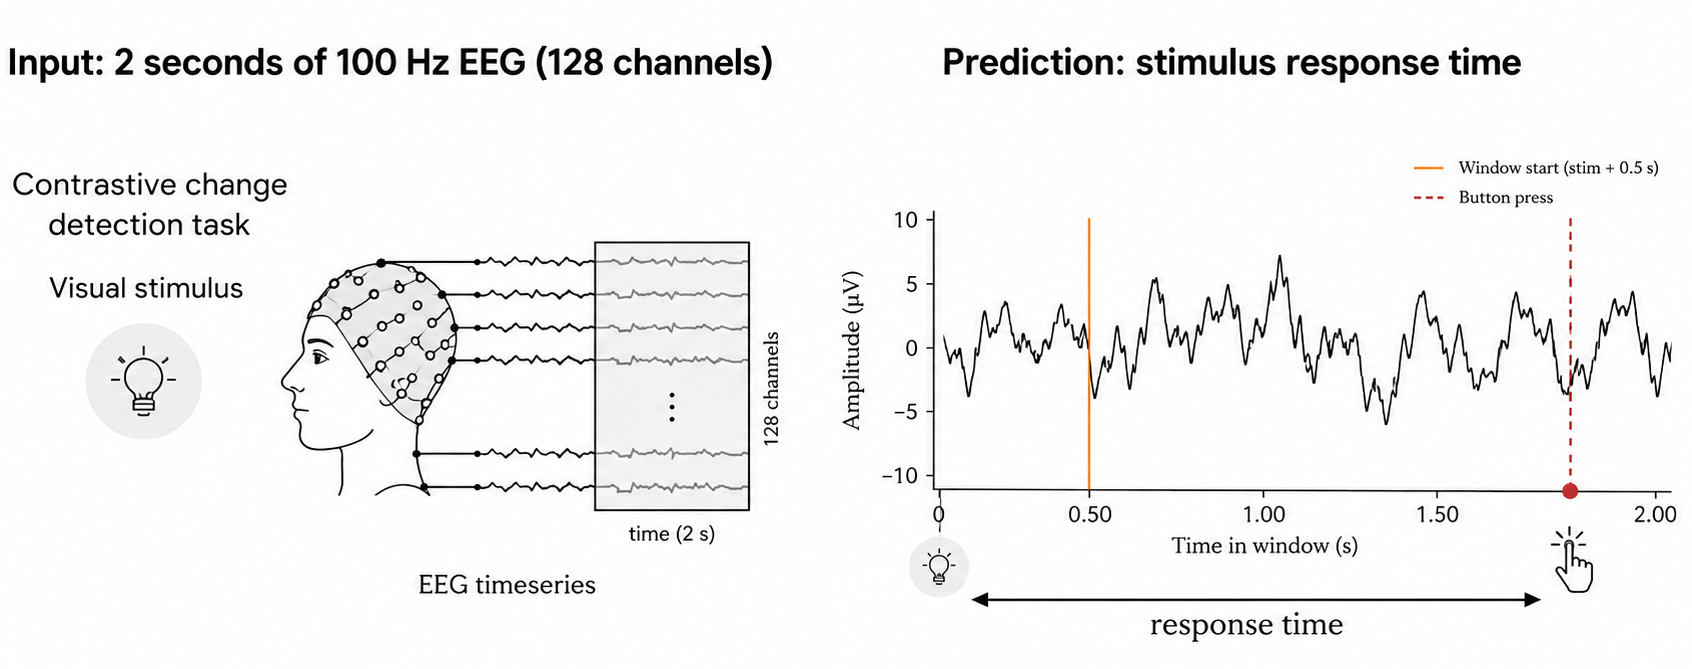
\includegraphics[width=0.9\linewidth]{img/challenge_task.png}
    \caption{HBN-EEG contrast change detection reaction-time task. Each trial provides a stimulus-locked EEG segment and a trial-wise RT target from stimulus onset to button press.}
    \label{fig:tasks}
\end{figure}


\subsection{Shared Evaluation Protocol}

We use this task as a controlled evaluation setting for separating three possible sources of RT prediction performance: EEG backbone capacity, temporal readout parameterization, and distributional event-time supervision. The benchmark therefore fixes the data split, target support, input representation, and scalar evaluation rule before varying architectures and objectives in the subsequent model and diagnostic sections.

To avoid subject leakage, all models use the same release-separated CCD split: R1--R8 for fitting, R9--R10 for development choices such as early stopping, checkpoint selection, readout-temperature tuning, and diagnostic settings for analyses that require them, and R11 for final holdout evaluation after all model and readout choices are fixed. R11 holdout labels are not used for model fitting, checkpoint selection, readout-temperature selection, or protocol decisions. Table~\ref{tab:ccd_protocol_stats} reports the resulting partitions; metadata checks confirmed zero subject overlap across train, development, and holdout after filtering.

\begin{table}[!t]
\centering
\caption{Release-separated CCD protocol statistics after window construction and RT-support filtering. Prepared trials are 2~s CCD windows with stimulus and response annotations; analyzed trials additionally satisfy \(0.5 \leq \mathrm{RT} \leq 2.5\)~s.}
\label{tab:ccd_protocol_stats}
\setlength{\tabcolsep}{3pt}
\renewcommand{\arraystretch}{1.12}
\begin{tabular*}{\linewidth}{@{\extracolsep{\fill}} l l r r r @{}}
\toprule
\textbf{Partition} & \textbf{Releases} & \textbf{Prepared trials} & \textbf{Analyzed trials} & \textbf{Subjects} \\
\midrule
Train & R1--R8 & 74{,}576 & 73{,}030 & 1{,}221 \\
Development & R9--R10 & 17{,}867 & 17{,}348 & 308 \\
Holdout & R11 & 15{,}751 & 15{,}164 & 292 \\
\bottomrule
\end{tabular*}
\end{table}

The main analysis keeps trials whose behavioral RT falls inside the modeled event-time support, 0.5--2.5~s after stimulus onset. This filter removes 1{,}546/74{,}576 training trials (2.07\%), 519/17{,}867 development trials (2.90\%), and 587/15{,}751 holdout trials (3.73\%). In the prepared CCD split, excluded trials are fast responses below 0.5~s; no prepared trial has RT above 2.5~s. The conclusions therefore apply to responses whose RT falls within the modeled post-stimulus support, and should not be interpreted as claims about very fast anticipatory responses or RT regimes outside the represented support.

Scalar performance is evaluated using normalized RMSE (nRMSE), defined as RMSE divided by the standard deviation of the true targets within the evaluated split \citep{EEGChallengeWebsite2025}. Main scalar comparisons use the same support-filtered R9--R10 development set and final holdout set. Diagnostic analyses that require shifted crop starts, stricter RT support, or posterior-only summaries are introduced in the corresponding subsection or appendix and do not affect the main holdout reporting protocol.

\begin{table}[!t]
\centering
\caption{Controlled comparison and diagnostic blocks under the shared protocol.}
\label{tab:experiment_map}
\scriptsize
\setlength{\tabcolsep}{2pt}
\renewcommand{\arraystretch}{1.08}
\begin{tabularx}{\linewidth}{@{} >{\RaggedRight\arraybackslash}p{0.21\linewidth} >{\RaggedRight\arraybackslash}p{0.18\linewidth} >{\RaggedRight\arraybackslash}p{0.18\linewidth} >{\RaggedRight\arraybackslash}X @{}}
\toprule
\textbf{Control or analysis} & \textbf{Readout} & \textbf{Supervision} & \textbf{Question addressed} \\
\midrule
\multicolumn{4}{@{}l}{\textit{Scalar regression controls}} \\
\addlinespace[0.15em]
External EEG backbones & Scalar RT head & Scalar RT & Does generic EEG backbone capacity explain performance? \\
MSP-CNN family & Segment-pooling scalar readout & Scalar RT & How far does coarse temporal pooling support scalar regression? \\
ETR-CNN family & Temporal expectation readout & Scalar RT & Does a learned temporal readout improve scalar regression? \\
\midrule
\multicolumn{4}{@{}l}{\textit{Event-time objective comparison with fixed ETS-U-Net}} \\
\addlinespace[0.15em]
Soft-argmax RT-loss control & Posterior mean & Scalar RT only & Is posterior-mean readout sufficient without distributional supervision? \\
CE soft-target objective & Posterior mean & Soft event-time target & Does direct distributional supervision improve RT prediction? \\
Likelihood-based objectives & Posterior mean & Latent event-time likelihood & Does probabilistic latent-event supervision provide the same benefit? \\
Wasserstein control & Posterior mean & Distributional geometry loss & Is an alternative geometry-based distributional objective sufficient? \\
\midrule
\multicolumn{4}{@{}l}{\textit{Architecture robustness controls}} \\
\addlinespace[0.15em]
ETS-TCN & Posterior mean & RT-only, CE, mixture EventNLL & Does the supervision effect persist with dilated temporal convolution? \\
ETS-InceptionPyramid & Posterior mean & RT-only, CE, mixture EventNLL & Does the supervision effect persist with multi-scale temporal filtering? \\
ETS-AttnSeg & Posterior mean & RT-only, CE, mixture EventNLL & Does the supervision effect persist with attention and local convolution? \\
\midrule
\multicolumn{4}{@{}l}{\textit{Posterior and localization diagnostics}} \\
\addlinespace[0.15em]
Readout-temperature tuning & Temperature-adjusted posterior mean & Learned posterior & How should the scalar posterior readout be standardized across objectives? \\
Posterior geometry diagnostics & Posterior summaries & Learned posterior & What posterior behavior is hidden by scalar nRMSE? \\
Shifted-crop diagnostic & Crop-relative posterior mean & No new training & Do predictions behave as crop-relative temporal localizers? \\
Shift-jitter intervention & Crop-relative posterior mean & Shifted crop-relative targets & Does crop-start augmentation reduce shortcut behavior? \\
\bottomrule
\end{tabularx}
\end{table}

Table~\ref{tab:experiment_map} maps the shared protocol to the comparison blocks used below. The scalar regression controls vary compact temporal regressors and external EEG backbones under scalar RT supervision. The event-time objective comparison fixes the ETS-U-Net backbone and varies the output supervision. The architecture-robustness comparison repeats a reduced objective set across different backbones. The primary and architecture-control models are described in Sections~\ref{sec:event_time_architectures} and~\ref{sec:architecture_robustness}, respectively. Posterior geometry, shifted-crop inference, and shift-jitter training are diagnostic extensions applied after training; they evaluate posterior semantics and shortcut-vs-localization behavior rather than defining a separate scalar benchmark family.

\subsection{Shared Training, Readout Tuning, and Inference Protocol}
\label{sec:shared_protocol}

To support the controlled comparison, we keep preprocessing, optimization, augmentation, checkpointing, and inference fixed across supervised neural models unless stated otherwise. Each 2~s trial window is normalized per channel by subtracting the channel's temporal mean within the window and dividing by its temporal standard deviation. The shared optimization and augmentation settings are summarized in Appendix~\ref{app:reproducibility_details}; in brief, models are trained with Adam, early stopping on development nRMSE, and a fixed augmentation profile combining channel dropout, temporal cutout, and Gaussian noise.

Regression models use scalar RT supervision, while event-time models represent RT either as a soft crop-relative event-time target or as an observation under a latent event-time likelihood. When temperature scaling is used for event-time posterior readout, \(\tau\) is selected on R9--R10 to minimize development nRMSE of the posterior-mean readout and then applied unchanged to the holdout split. The main regression-baseline and event-time-objective comparisons are repeated over five seeds (2025--2029), and repeated-run tables report mean $\pm$ standard deviation across seeds unless otherwise stated.

\section{Scalar Regression Controls}
\label{sec:baseline_regression}

Before introducing event-time targets, we first ask how far scalar RT supervision can go under the same release-separated protocol. The regression baselines use compact task-specific temporal regressors as strong scalar controls and external EEG backbones as architecture-capacity controls.

The compact controls form a progression of window-level temporal inductive biases. MSP-CNN (multiscale segment-statistic pooling CNN; Figure~\ref{fig:ch1_regression}) explicitly accounts for temporal structure by collecting mean and max statistics from coarse temporal segments of the feature map. These segment-level summaries act as early/middle/late activation cues and are mapped to scalar RT. ETR-CNN (event-time readout CNN) turns this coarse temporal summary into a learned time-indexed readout: it preserves temporal scores over the input window and predicts RT as the expected time under learned time-bin weights. ETR-CNN large keeps the same readout while increasing feature capacity.

We compare these task-specific regressors with external EEG architectures adapted to scalar RT regression. These include classical convolutional EEG baselines, Deep4Net and ShallowFBCSPNet \citep{braindecode}; the compact EEGNet architecture \citep{lawhern2018eegnet}; TIDNet's thinker-invariant convolutional design \citep{kostas2020thinkerinvariance}; the convolutional-transformer EEGConformer \citep{song2023eegconformer}; the attention temporal convolutional ATCNet architecture \citep{altaheri2022atcnet}; EEGPT \citep{wang2024eegpt}; Medformer \citep{wang2024medformer}; and the LaBraM foundation-style architecture \citep{Jiang2024LaBraM}. All external architectures are trained from scratch; pretrained weights are not used.

ETR-CNN large is the strongest scalar baseline, with MSP-CNN and base ETR-CNN close behind. The external EEG backbones train successfully under this protocol but do not close the gap to these compact temporal controls, suggesting that task-specific temporal structure matters more for this RT task than generic backbone capacity alone. These results provide strong scalar controls for the next step: testing whether directly supervising an event-time distribution improves beyond scalar RT training.

\begin{figure}[!t]
    \centering
    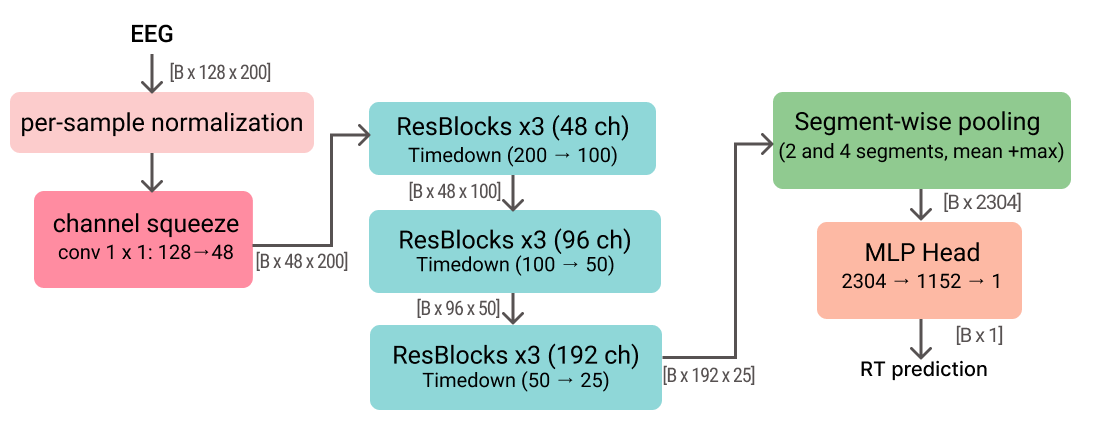
\includegraphics[width=\linewidth]{img/ch1/Ch1_regression.png}
    \caption{MSP-CNN direct RT regression baseline architecture. A lightweight 1-D temporal ConvNet maps an EEG trial window to a scalar reaction-time prediction. A learned $1\times1$ channel-squeeze layer (128$\rightarrow$48) is followed by residual depthwise-separable stages with anti-aliased temporal downsampling, segment-wise pooling (2 and 4 segments; mean+max), and an MLP head.}
    \label{fig:ch1_regression}
\end{figure}

\begin{table}[!t]
\centering
\caption{Direct-regression and external backbone baselines.}
\label{tab:r11_regression_baselines}
\footnotesize
\setlength{\tabcolsep}{2pt}
\renewcommand{\arraystretch}{1.15}
\begin{tabularx}{\linewidth}{@{} >{\RaggedRight\arraybackslash}p{0.22\linewidth} Y >{\centering\arraybackslash}p{0.215\linewidth} >{\centering\arraybackslash}p{0.215\linewidth} @{}}
\toprule
\textbf{Model} & \textbf{Role} & \textbf{Valid nRMSE} $\downarrow$ & \textbf{Holdout nRMSE} $\downarrow$ \\
\midrule
\multicolumn{4}{@{}l}{\textit{Task-specific regression baselines}} \\
\addlinespace[0.15em]
MSP-CNN & segment-pooling scalar & \mbox{0.9006 $\pm$ 0.0051} & \mbox{0.8998 $\pm$ 0.0080} \\
ETR-CNN & temporal readout & \mbox{0.9008 $\pm$ 0.0060} & \mbox{0.8977 $\pm$ 0.0068} \\
ETR-CNN large & capacity ablation & \textbf{\mbox{0.8972 $\pm$ 0.0040}} & \textbf{\mbox{0.8928 $\pm$ 0.0042}} \\
\midrule
\multicolumn{4}{@{}l}{\textit{External regression baselines}} \\
\addlinespace[0.15em]
TIDNet & thinker-invariant CNN & \mbox{0.9235 $\pm$ 0.0024} & \textbf{\mbox{0.9192 $\pm$ 0.0027}} \\
EEGConformer & conv-transformer & \textbf{\mbox{0.9188 $\pm$ 0.0026}} & \mbox{0.9287 $\pm$ 0.0057} \\
EEGNet & compact CNN & \mbox{0.9350 $\pm$ 0.0054} & \mbox{0.9335 $\pm$ 0.0028} \\
LaBraM & foundation-style & \mbox{0.9304 $\pm$ 0.0061} & \mbox{0.9327 $\pm$ 0.0086} \\
Deep4Net & deep ConvNet & \mbox{0.9269 $\pm$ 0.0045} & \mbox{0.9260 $\pm$ 0.0044} \\
ShallowFBCSPNet & shallow FBCSP CNN & \mbox{0.9324 $\pm$ 0.0016} & \mbox{0.9343 $\pm$ 0.0024} \\
ATCNet & conv/attention/TCN & \mbox{0.9686 $\pm$ 0.0183} & \mbox{0.9666 $\pm$ 0.0151} \\
EEGPT & foundation-style & \mbox{0.9616 $\pm$ 0.0201} & \mbox{0.9584 $\pm$ 0.0185} \\
Medformer & larger transformer & \mbox{0.9623 $\pm$ 0.0046} & \mbox{0.9585 $\pm$ 0.0051} \\
\bottomrule
\end{tabularx}
\end{table}

\section{Event-Time Posterior Formulation}
\label{sec:event_time_formulation}

To make response timing explicit, we reformulate RT prediction as event-time posterior modeling. Instead of predicting a scalar directly, the model produces per-time logits and a posterior distribution over response-relevant event times; scalar RT is then read out as the posterior expectation. The key distinction from temporal-readout regression is that the objective directly supervises the distributional event-time representation, rather than using a temporal head only as a scalar-regression readout.

We evaluate two ways of converting scalar RT labels into event-time supervision. The first constructs an explicit soft target distribution over time, asking the model to match a smoothed target centered at the observed RT. The second treats the observed RT statistically, as a noisy observation of an unobserved response-relevant event time, and optimizes a latent event-time likelihood. These two families correspond to soft-target objectives and likelihood-based objectives, respectively.

The core event-time experiments are organized as a primary controlled comparison
and a secondary architecture-robustness analysis. The regression controls above quantify
what scalar supervision achieves with task-specific temporal readouts and external EEG
backbones.

We use the event-time segmentation U-Net (ETS-U-Net) as the primary backbone
for the objective comparisons because its dense temporal segmentation design
naturally matches the event-time output space: it maps each EEG window to
per-time logits while combining local and broader temporal context through an
encoder--decoder path with skip connections. Fixing this backbone allows us to
isolate the effect of output supervision under a strong segmentation model.
Additional dense temporal backbones then test whether the resulting supervision
effects persist beyond the U-Net inductive bias, as described in
Section~\ref{sec:architecture_robustness}.

\begin{figure}[!t]
    \centering
    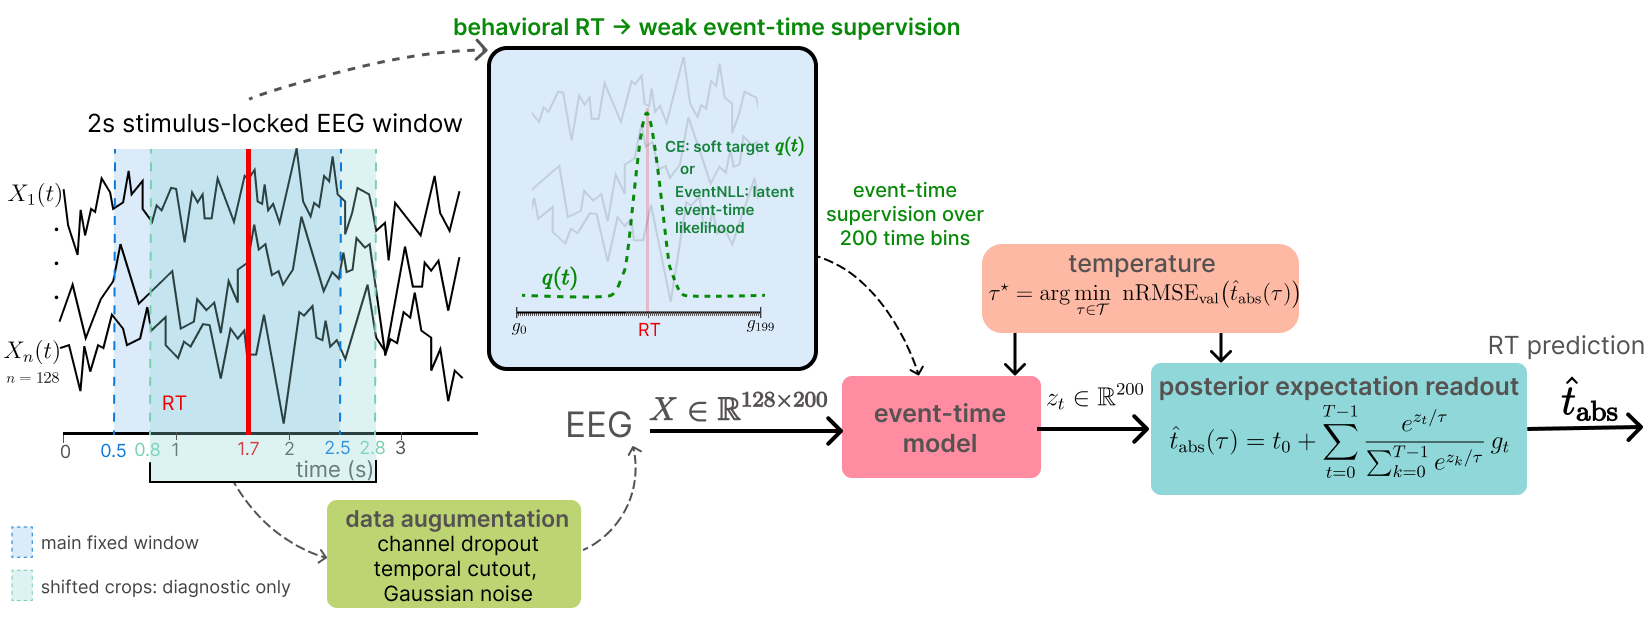
\includegraphics[width=\linewidth]{img/ch1/event_time_scheme.png}
    \caption{Event-time posterior formulation for EEG reaction-time prediction. A fixed 0.5--2.5~s stimulus-locked EEG window is mapped to time-bin logits, and behavioral RT provides weak event-time supervision either through a soft target distribution or a latent EventNLL likelihood. Scalar RT is read out as the posterior expectation after selecting a readout temperature on R9--R10. Shifted crops are used only for diagnostic and shift-jitter intervention analyses. The schematic shows the categorical posterior readout; the hazard EventNLL variant uses a hazard-derived probability mass function with the same expectation readout.}
    \label{fig:event_time_scheme}
\end{figure}

\subsection{Primary Event-Time Segmentation Architecture}
\label{sec:event_time_architectures}

ETS-U-Net maps an EEG trial window
$X\in\mathbb{R}^{C\times T}$ to per-time logits $z_{0:T-1}$ (Figure~\ref{fig:ets_unet}). It follows a 1-D U-Net style encoder-decoder with skip
connections for precise localization \citep{ronneberger2015unet}. The encoder progressively downsamples the temporal axis
to build multi-scale context, while the decoder upsamples and fuses encoder features to recover per-time outputs at the
input temporal resolution (downsampling and upsampling are used only to form multi-scale features). Each scale is refined
with lightweight residual blocks (ResNet-style skips) \citep{he2016resnet} built from depthwise-separable 1-D convolutions
for computational efficiency \citep{howard2017mobilenets,chollet2017xception}. To mitigate aliasing under temporal
decimation, downsampling applies a fixed depthwise smoothing filter followed by strided averaging (``blur-pool'' style)
\citep{zhang2019shiftinvariant}. A dilated bottleneck further enlarges the receptive field without additional downsampling
\citep{yu2016dilated}.

\begin{figure}[t]
    \centering
    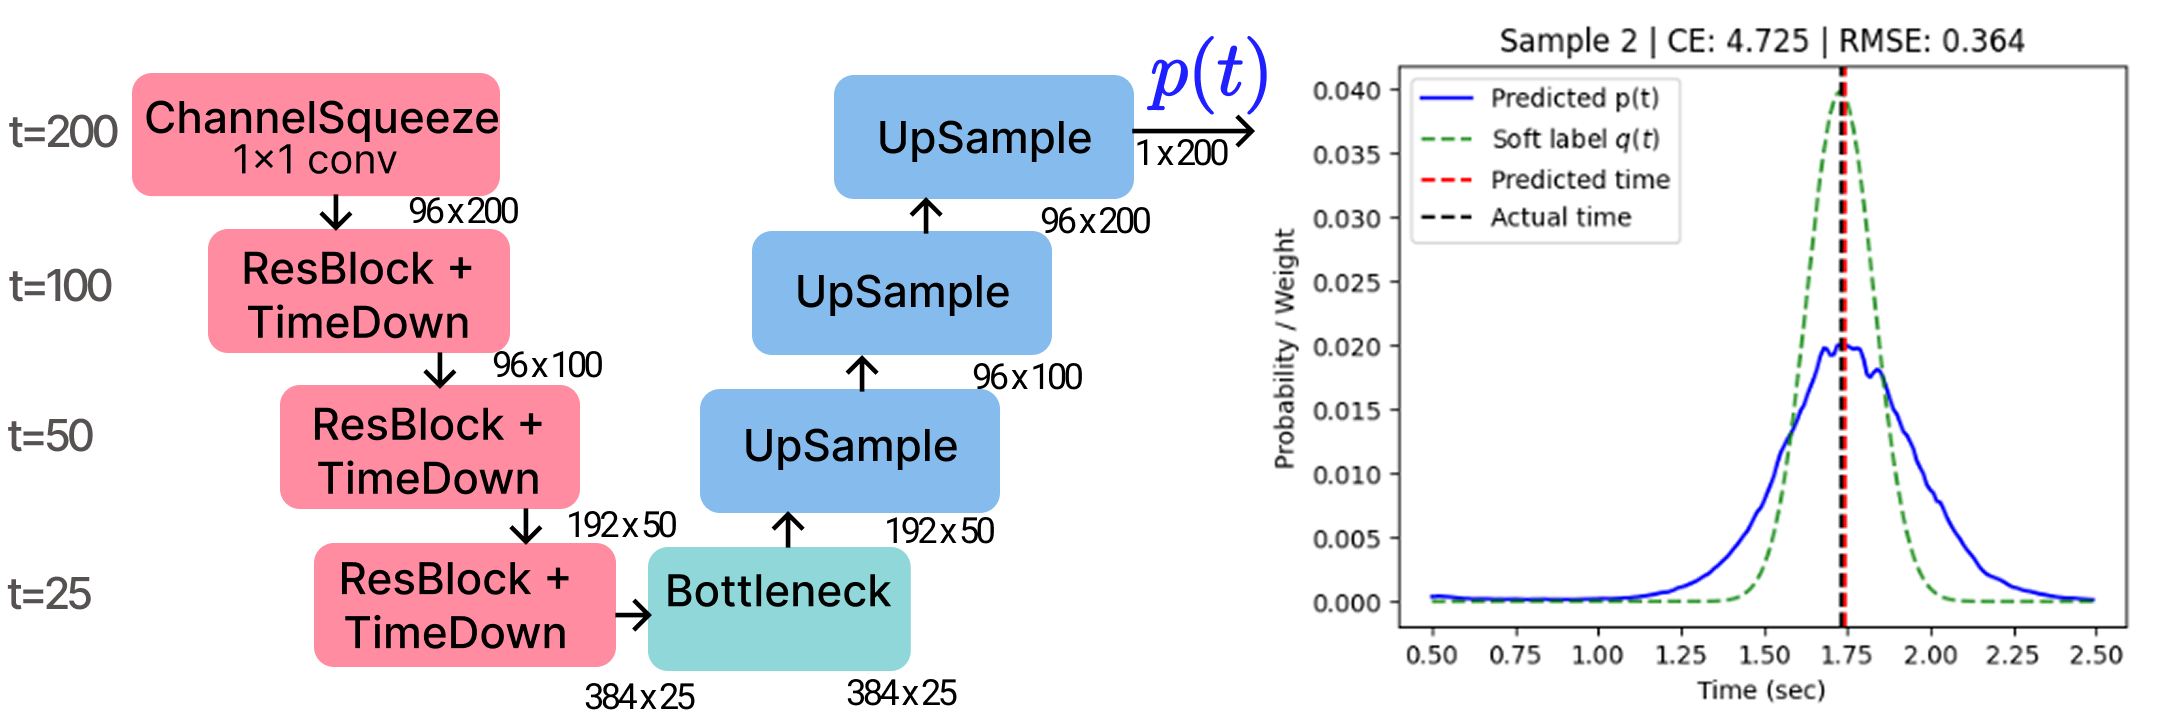
\includegraphics[width=0.9\linewidth]{img/ch1/Ch1_ets_unet_1.png}
    \caption{ETS-U-Net for RT segmentation. A lightweight 1-D U-Net maps an EEG trial window to per-time logits
    and an event-time distribution $p(t)$. The encoder applies a $1\times1$ channel-squeeze layer followed by residual
    blocks with temporal downsampling (\texttt{TimeDown}); a bottleneck aggregates context, and the decoder upsamples with
    skip connections to recover time-resolved outputs. The right panel shows an example prediction $p(t)$ and Gaussian soft
    target $q(t)$, together with the resulting predicted vs.\ observed response time.}
    \label{fig:ets_unet}
\end{figure}

\subsection{Soft-Target Event-Time Objectives}

Soft-target objectives provide direct supervision by converting the observed RT into a smooth target distribution over the represented time grid.

\paragraph{Soft target distribution.}
For each fixed 2~s input window, the observed RT \(y\) is converted into a
window-relative temporal target \(y_{\mathrm{rel}}=y-0.5\)~s on the represented
time grid.
A smooth segmentation label is constructed using a Gaussian kernel with bandwidth $\sigma$:
\begin{equation}
\label{eq:rt_soft_target}
\tilde q_t=\exp\left(-\frac{(g_t-y_{\mathrm{rel}})^2}{2\sigma^2}\right),\qquad
q_t=\frac{\tilde q_t}{\sum_{k=0}^{T-1}\tilde q_k},\qquad
\sum_{t=0}^{T-1} q_t=1.
\end{equation}
The Gaussian label avoids a degenerate single-bin target while keeping probability mass concentrated near the observed behavioral latency.

\paragraph{Model output and losses.}
Given logits $z_t$ for $t=0,\dots,T-1$, the predicted event-time distribution is obtained via temperature-scaled softmax,
\begin{equation}
\label{eq:rt_pred_dist}
p_t(\tau)=\frac{e^{z_t/\tau}}{\sum_{k=0}^{T-1} e^{z_k/\tau}}.
\end{equation}
The soft-label segmentation family is written as a weighted objective:
\begin{equation}
\label{eq:rt_loss}
\begin{aligned}
\mathcal{L}
&= \lambda_{\text{time}}\,\mathrm{RMSE}\big(\hat t_{\mathrm{rel}}(\tau), y_{\mathrm{rel}}\big)
 + \lambda_{\text{CE}}\,\mathrm{CE}\big(q, p(\tau)\big) \\
&\quad + \lambda_{W1}\,W_1\big(\mathrm{CDF}(q), \mathrm{CDF}(p(\tau))\big)
 + \lambda_{\text{KL}}\,D_{\mathrm{KL}}\big(q\|p(\tau)\big)
 + \lambda_{H}\,H\big(p(\tau)\big),
\end{aligned}
\end{equation}
where  
\begin{equation*}
\mathrm{CE}(q,p)=-\sum_{t=0}^{T-1} q_t \log p_t, \;
D_{\mathrm{KL}}(q\|p)=\sum_{t=0}^{T-1} q_t \log\frac{q_t}{p_t}, \;
H(p)=-\sum_{t=0}^{T-1} p_t \log p_t.
\end{equation*}
This expression defines an ablation family rather than a single prescribed loss. CE-only supervision sets the scalar time term to zero and asks the model to match a Gaussian soft event-time label. The soft-argmax RT-loss ablation removes distributional matching while keeping the same readout, and the Wasserstein-only ablation tests whether a CDF-based geometry loss is sufficient on its own. A CE+time hybrid combines both CE and soft-argmax time terms, but is not reported as a separate row in the five-seed comparison. Entropy, KL, focal, and related terms serve as posterior-geometry controls when included.

\subsection{Likelihood-Based Event-Time Objectives}
\label{sec:event_nll}

As a probabilistic alternative to soft-target supervision, likelihood-based objectives model the observed scalar RT as a noisy realization of a latent response-relevant event time. Given the posterior over latent event bins, the marginal likelihood of the observed RT is
\begin{equation}
\label{eq:event_nll}
p(y\mid X)
= \sum_{t=0}^{T-1} p_t(X)\,
\mathcal{N}\!\left(y;\,t_0 + g_t,\,\sigma_y^2\right),
\qquad
\mathcal{L}_{\mathrm{EventNLL}} = -\log p(y\mid X).
\end{equation}
This objective keeps the same event-time interpretation but replaces the constructed target distribution $q_t$ with a marginal likelihood over latent response-relevant event times.

\paragraph{Observation-kernel and hazard extensions.}
The EventNLL formulation separates the latent event-time posterior $p_t(X)$ from the observation model $K(y\mid t)$. The posterior/observation-kernel separation is also consistent with measurement-oriented views of learned representations as proxy measurements of latent variables \citep{Yao2025ThirdPillar}. The default model uses a single Gaussian observation kernel, but we also evaluate a two-scale Gaussian mixture,
\begin{equation}
\label{eq:event_nll_mixture_kernel}
K(y\mid t)=(1-\alpha)\,\mathcal{N}(y;t_0+g_t,\sigma_{\mathrm{narrow}}^2)
+\alpha\,\mathcal{N}(y;t_0+g_t,\sigma_{\mathrm{wide}}^2),
\end{equation}
which keeps most probability mass in a narrow timing error while allowing a wider tail for occasional noisy RT observations. In these experiments, $\sigma_{\mathrm{narrow}}=0.10$~s, $\sigma_{\mathrm{wide}}=0.35$~s, and $\alpha=0.10$.

As a readout extension, we also evaluate a hazard/survival parameterization. Instead of using logits only as unconstrained softmax scores, each temporal logit defines a conditional event probability
\begin{equation}
\label{eq:hazard_readout}
h_t=\sigma(z_t/\tau),\qquad
p_t^{\mathrm{haz}} \propto h_t\prod_{k<t}(1-h_k),
\end{equation}
with the resulting event-bin probabilities normalized over the represented window. This keeps the same event-time likelihood in Eq.~\ref{eq:event_nll}, but changes the posterior parameterization from a categorical softmax to a discrete-time survival process. This extension tests whether the event-time formulation depends on a particular softmax parameterization.

\subsection{Formulation Comparison and Robustness}

This comparison asks whether the event-time formulation improves RT prediction because it changes the supervised output distribution, rather than simply because it adds a temporal posterior readout. Table~\ref{tab:r11_segmentation_losses} evaluates the reported ETS-U-Net objective variants under the fixed backbone and release-separated protocol. Holdout \(\tau\)-nRMSE denotes holdout nRMSE after applying the posterior-readout temperature \(\tau\) selected on R9--R10; holdout labels are used only for evaluation. The CE and likelihood-family objectives form the strongest scalar-readout group after readout-temperature tuning, with holdout \(\tau\)-nRMSE between 0.8745 and 0.8778. This improves over the strongest scalar regression baseline, ETR-CNN large (0.8928 $\pm$ 0.0042; Table~\ref{tab:r11_regression_baselines}), whereas the soft-argmax RT-loss and Wasserstein controls remain closer to the scalar-regression baselines.

This is a conservative comparison because ETR-CNN large already includes a task-specific temporal expectation readout rather than a generic scalar head. The improvement is larger relative to scalar baselines without this specialized temporal readout, but the stronger point is that event-time supervision still adds value after strong scalar temporal inductive biases are included.

\begin{table}[!htbp]
\centering
\caption{Event-time objective variants with a fixed ETS-U-Net backbone. Temperature is selected on R9--R10 for posterior-mean readout and then applied unchanged to the holdout split.}
\label{tab:r11_segmentation_losses}
\footnotesize
\setlength{\tabcolsep}{2pt}
\renewcommand{\arraystretch}{1.15}
\begin{tabularx}{\linewidth}{@{} >{\RaggedRight\arraybackslash}p{0.18\linewidth} Y >{\centering\arraybackslash}p{0.17\linewidth} >{\centering\arraybackslash}p{0.17\linewidth} >{\centering\arraybackslash}p{0.17\linewidth} @{}}
\toprule
\textbf{Objective} & \textbf{Supervision signal} & \textbf{Valid nRMSE} & \textbf{Holdout nRMSE} & \textbf{Holdout \(\tau\)-nRMSE} \\
\midrule
\multicolumn{5}{@{}l}{\textit{Soft-target objectives}} \\
\addlinespace[0.15em]
CE & Gaussian soft event-time label & \mbox{0.8763 $\pm$ 0.0044} & \textbf{\mbox{0.8774 $\pm$ 0.0044}} & \mbox{0.8753 $\pm$ 0.0039} \\
\midrule
\multicolumn{5}{@{}l}{\textit{Likelihood-based objectives}} \\
\addlinespace[0.15em]
EventNLL & latent event time + Gaussian RT likelihood & \mbox{0.8769 $\pm$ 0.0030} & \mbox{0.8805 $\pm$ 0.0021} & \mbox{0.8772 $\pm$ 0.0018} \\
Mixture EventNLL & Two-component core-tail RT likelihood & \textbf{\mbox{0.8744 $\pm$ 0.0018}} & \mbox{0.8785 $\pm$ 0.0047} & \textbf{\mbox{0.8745 $\pm$ 0.0053}} \\
Hazard EventNLL & hazard posterior + Gaussian RT likelihood & \mbox{0.8755 $\pm$ 0.0027} & \mbox{0.8776 $\pm$ 0.0031} & \mbox{0.8778 $\pm$ 0.0041} \\
\midrule
\multicolumn{5}{@{}l}{\textit{Scalar-readout and distance controls}} \\
\addlinespace[0.15em]
Soft-argmax RT loss & posterior-mean RT error only; no distribution target & \mbox{0.8944 $\pm$ 0.0048} & \mbox{0.8943 $\pm$ 0.0025} & \mbox{0.8917 $\pm$ 0.0046} \\
Wasserstein & CDF match to Gaussian soft event-time label & \mbox{0.8997 $\pm$ 0.0035} & \mbox{0.8995 $\pm$ 0.0078} & \mbox{0.8896 $\pm$ 0.0033} \\
\bottomrule
\end{tabularx}
\end{table}
\FloatBarrier

\paragraph{Objective ablations.}
The ablations separate expectation-style temporal readout from distributional supervision. The soft-argmax RT-loss control directly optimizes posterior-mean RT error but removes distribution matching; it remains close to the strongest scalar-regression baseline and trails the CE/EventNLL group by roughly 0.014--0.017 holdout \(\tau\)-nRMSE. CE and the likelihood-family variants form a tight cluster among the best-performing objectives: mixture EventNLL has the best mean temperature-tuned scalar readout, but CE, Gaussian EventNLL, mixture EventNLL, and hazard EventNLL are close relative to seed variability. The hazard result shows that the likelihood-family conclusion is not tied to a categorical softmax posterior, while the Wasserstein control shows that an alternative distributional distance alone does not match the CE/EventNLL scalar readouts. Within the fixed ETS-U-Net backbone, these results isolate the gain to the supervision objective rather than to the temporal expectation readout alone. The next subsection tests whether the same supervision pattern persists when the dense temporal backbone is changed.

\paragraph{Practical effect size.}
To express the main accuracy gain on the RT scale, we compared the strongest scalar baseline, ETR-CNN large, with the strongest event-time objectives using matched seeds and subject-level bootstrap intervals on the holdout split. Mixture EventNLL reduced \(\tau\)-nRMSE from \(0.8928 \pm 0.0042\) to \(0.8745 \pm 0.0053\), an absolute reduction of \(0.0184\), or about \(2.1\%\) relative improvement. On the RT scale, this corresponds to a \(6.24\)~ms reduction in RMSE and an \(8.94\)~ms reduction in MAE, with subject-bootstrap 95\% confidence intervals of \([4.50, 7.97]\)~ms and \([7.43, 10.49]\)~ms, respectively. The gain was positive for all five matched-seed comparisons. Thus, even against a strong temporal-readout scalar baseline, the scalar accuracy gain is modest in absolute terms but consistent across seeds and subjects. The event-time formulation also provides posterior diagnostics and shifted-crop analyses that are not available from scalar regression alone.

\begin{figure}[!t]
    \centering
    
\includegraphics[width=0.88\linewidth]{img/ch1/trial_sorted_posterior_raster.png}
    \caption{Trial-sorted event-time posterior maps on the holdout split for matched segmentation losses. Rows are quantile bins of representable holdout trials sorted by observed RT; the x-axis is time from stimulus onset; color shows log-transformed posterior density averaged within each bin. The overlaid curve marks the mean observed RT in each bin.}
    \label{fig:posterior_raster_main}
\end{figure}

\subsection{Architecture Robustness of the Supervision Effect}
\label{sec:architecture_robustness}

To assess whether the supervision effect is robust to backbone choice, we
repeat the RT-only soft-argmax, CE, and mixture EventNLL comparison using three
custom temporal backbones. These controls preserve full-resolution event-time
output, closely match ETS-U-Net in capacity, and span three distinct temporal
inductive biases.

ETS-TCN uses residual dilated temporal convolutions
\citep{bai2018tcn,yu2016dilated}. ETS-InceptionPyramid applies parallel
depthwise temporal filters at multiple receptive-field scales and fuses them
through residual blocks, following Inception-style design principles
\citep{szegedy2015going,santamaria2020eeginception}. ETS-AttnSeg uses
Conformer-style blocks that combine global temporal self-attention with local
gated depthwise convolution
\citep{vaswani2017attention,gulati2020conformer}. The three controls contain
3.05--3.25 million trainable parameters, compared with 3.10 million for
ETS-U-Net.

Table~\ref{tab:architecture_robustness} reports the resulting scalar RT
comparison.

\begin{table}[!htbp]
\centering
\caption{Scalar RT accuracy across matched dense temporal backbones and supervision objectives.}
\label{tab:architecture_robustness}
\footnotesize
\setlength{\tabcolsep}{3pt}
\renewcommand{\arraystretch}{1.15}
\begin{tabularx}{\linewidth}{@{} Y >{\centering\arraybackslash}p{0.22\linewidth} >{\centering\arraybackslash}p{0.22\linewidth} >{\centering\arraybackslash}p{0.22\linewidth} @{}}
\toprule
\textbf{Objective} & \textbf{Valid nRMSE} & \textbf{Holdout nRMSE} & \textbf{Holdout $\tau$-nRMSE} \\
\midrule
\multicolumn{4}{@{}l}{\textit{ETS-U-Net}} \\
\addlinespace[0.15em]
RT-only soft-argmax & \mbox{0.8944 $\pm$ 0.0048} & \mbox{0.8943 $\pm$ 0.0025} & \mbox{0.8917 $\pm$ 0.0046} \\
CE & \mbox{0.8763 $\pm$ 0.0044} & \mbox{0.8774 $\pm$ 0.0044} & \mbox{0.8753 $\pm$ 0.0039} \\
Mixture EventNLL & \mbox{0.8744 $\pm$ 0.0018} & \mbox{0.8785 $\pm$ 0.0047} & \textbf{\mbox{0.8745 $\pm$ 0.0053}} \\
\midrule
\multicolumn{4}{@{}l}{\textit{ETS-TCN}} \\
\addlinespace[0.15em]
RT-only soft-argmax & \mbox{0.8865 $\pm$ 0.0029} & \mbox{0.8853 $\pm$ 0.0044} & \mbox{0.8842 $\pm$ 0.0045} \\
CE & \mbox{0.8717 $\pm$ 0.0025} & \mbox{0.8751 $\pm$ 0.0085} & \mbox{0.8730 $\pm$ 0.0038} \\
Mixture EventNLL & \mbox{0.8718 $\pm$ 0.0046} & \mbox{0.8729 $\pm$ 0.0020} & \textbf{\mbox{0.8722 $\pm$ 0.0021}} \\
\midrule
\multicolumn{4}{@{}l}{\textit{ETS-InceptionPyramid}} \\
\addlinespace[0.15em]
RT-only soft-argmax & \mbox{0.8970 $\pm$ 0.0043} & \mbox{0.8894 $\pm$ 0.0054} & \mbox{0.8886 $\pm$ 0.0044} \\
CE & \mbox{0.8710 $\pm$ 0.0037} & \mbox{0.8717 $\pm$ 0.0017} & \textbf{\mbox{0.8717 $\pm$ 0.0036}} \\
Mixture EventNLL & \mbox{0.8703 $\pm$ 0.0018} & \mbox{0.8780 $\pm$ 0.0026} & \mbox{0.8746 $\pm$ 0.0028} \\
\midrule
\multicolumn{4}{@{}l}{\textit{ETS-AttnSeg}} \\
\addlinespace[0.15em]
RT-only soft-argmax & \mbox{0.9114 $\pm$ 0.0350} & \mbox{0.9105 $\pm$ 0.0294} & \mbox{0.9052 $\pm$ 0.0300} \\
CE & \mbox{0.8742 $\pm$ 0.0036} & \mbox{0.8811 $\pm$ 0.0097} & \mbox{0.8780 $\pm$ 0.0082} \\
Mixture EventNLL & \mbox{0.8719 $\pm$ 0.0082} & \mbox{0.8823 $\pm$ 0.0079} & \textbf{\mbox{0.8752 $\pm$ 0.0050}} \\
\bottomrule
\end{tabularx}
\end{table}
\FloatBarrier

Across all four backbones, both CE and mixture EventNLL yield lower mean
holdout $\tau$-nRMSE than the RT-only soft-argmax control. Their ordering is
not uniform: mixture EventNLL has the lower mean for ETS-U-Net, ETS-TCN, and
ETS-AttnSeg, whereas CE has the lower mean for ETS-InceptionPyramid. Taken
together, these results show that distributional supervision yields lower error
than RT-only posterior-mean training across distinct backbone designs. This
pattern is therefore not specific to ETS-U-Net.
Complementary shifted-crop and posterior-geometry controls are reported in
Appendix~\ref{app:architecture_controls}.

\section{Posterior Readout and Diagnostics}
\label{sec:posterior_diagnostics}

\subsection{Scalar Readout and Temperature Tuning}

\paragraph{Posterior-mean scalar readout.}
Event-time models output a posterior over response-relevant time bins, whereas the benchmark evaluates scalar RT. We therefore use the posterior expectation as the scalar readout: the predicted relative time is the probability-weighted average of the temporal grid, and the absolute RT is obtained by adding the fixed window start time,
\begin{equation}
\label{eq:rt_soft_argmax}
\hat t_{\mathrm{rel}}(\tau)=\sum_{t=0}^{T-1} p_t(\tau)\, g_t,
\qquad
\hat t_{\mathrm{abs}}(\tau)=t_0+\hat t_{\mathrm{rel}}(\tau),
\end{equation}
where $g_t=t\,\Delta t$ denotes the discrete time grid. This readout is aligned with squared-error evaluation and keeps event-time models comparable to scalar regression baselines under nRMSE.

\paragraph{Readout-temperature tuning.}
Because different objectives can produce posteriors with different sharpness, we select a readout temperature on the R9--R10 development split to minimize nRMSE of the posterior-mean prediction, and apply the selected temperature unchanged to the holdout set:
\begin{equation}
\label{eq:rt_tau_tuning}
\tau_m^\star = \arg\min_{\tau\in\mathcal{T}_{\text{cal}}}
\ \mathrm{nRMSE}_{\text{val}}\big(\hat t_{\mathrm{abs}}^{(m)}(\tau)\big).
\end{equation}
The resulting scalar value is reported as holdout \(\tau\)-nRMSE in Table~\ref{tab:r11_segmentation_losses}. This temperature step is a scalar-readout protocol, not a full probabilistic calibration; likelihood, coverage, and posterior concentration are evaluated separately below.

\begin{figure}[!t]
    \centering
    
\includegraphics[width=\linewidth]{img/ch1/posterior_geometry_main.png}
    \caption{Posterior geometry differs across event-time losses even when scalar nRMSE is similar. Panel A reports holdout scalar readout after selecting the softmax temperature on R9--R10 to minimize nRMSE. Panel B aligns predicted posteriors to the observed RT. Panels C--E summarize posterior width, near-target mass, and mode-mean disagreement. Panel F compares empirical coverage of central posterior intervals; the diagonal is ideal interval coverage.}
    \label{fig:posterior_geometry_main}
\end{figure}

\subsection{Posterior Geometry Diagnostics}

Once the scalar readout has been fixed, the event-time posterior makes temporally resolved evaluation possible rather than limiting assessment to point prediction. Scalar nRMSE asks whether the posterior mean predicts RT accurately, but similar nRMSE values can hide very different temporal evidence. Posterior-geometry diagnostics quantify where probability mass is placed, whether it is localized near the observed behavioral latency, whether the posterior peak agrees with the posterior mean, and whether nominal posterior intervals have meaningful empirical coverage.

We first inspect the trial-sorted posterior maps in Figure~\ref{fig:posterior_raster_main} before reducing the posterior to summary metrics. These maps show the full distribution over response-relevant event time for holdout trials ordered by observed RT, rather than only the posterior mean. CE and Wasserstein place broad probability mass across the response window, whereas the EventNLL-family objectives produce sharper probability bands that more closely track the observed RT curve. This qualitative pattern motivates the quantitative posterior-geometry summaries in Figure~\ref{fig:posterior_geometry_main} and Table~\ref{tab:posterior_geometry_metrics}.

Figure~\ref{fig:posterior_geometry_main} visualizes these posterior summaries, and Table~\ref{tab:posterior_geometry_metrics} reports the corresponding quantitative values. The six diagnostics separate complementary properties of the posterior: posterior-mean scalar accuracy (nRMSE), distributional scoring under a common observation kernel (fixed-kernel EventNLL), concentration and target alignment (Width80 and Mass $\pm$150 ms), and empirical interval behavior (Coverage80 and Coverage MAE). Together, they define a trade-off space in which similar scalar errors can correspond to different temporal posterior behavior.

\begin{table}[!htbp]
\centering
\caption{Quantitative posterior geometry on the holdout split for matched event-time segmentation losses. Values are mean $\pm$ standard deviation across seeds after R9--R10 readout-temperature selection; arrows indicate the preferred direction, Coverage80 is best when close to 0.80, and bold marks the best point estimate per metric.}
\label{tab:posterior_geometry_metrics}
\scriptsize
\setlength{\tabcolsep}{3pt}
\renewcommand{\arraystretch}{1.12}
\resizebox{\linewidth}{!}{%
\begin{tabular}{@{} l c c c c c c @{}}
\toprule
\textbf{Objective} & \textbf{nRMSE $\downarrow$} & \textbf{Fixed-kernel EventNLL $\downarrow$} & \textbf{Width80 ms $\downarrow$} & \textbf{Mass $\pm$150 ms $\uparrow$} & \textbf{Coverage80} & \textbf{Coverage MAE $\downarrow$} \\
\midrule
CE & 0.875 $\pm$ 0.004 & 0.08 $\pm$ 0.01 & 766 $\pm$ 36 & 0.334 $\pm$ 0.008 & 0.883 $\pm$ 0.013 & 0.101 $\pm$ 0.014 \\
EventNLL & 0.877 $\pm$ 0.002 & -0.06 $\pm$ 0.01 & 502 $\pm$ 15 & 0.490 $\pm$ 0.008 & 0.500 $\pm$ 0.025 & 0.273 $\pm$ 0.021 \\
Mixture EventNLL & \textbf{0.874 $\pm$ 0.005} & \textbf{-0.08 $\pm$ 0.01} & 528 $\pm$ 22 & 0.471 $\pm$ 0.008 & 0.573 $\pm$ 0.020 & 0.207 $\pm$ 0.017 \\
Hazard EventNLL & 0.878 $\pm$ 0.004 & -0.06 $\pm$ 0.01 & \textbf{445 $\pm$ 14} & \textbf{0.502 $\pm$ 0.005} & 0.468 $\pm$ 0.007 & 0.302 $\pm$ 0.006 \\
Soft-argmax RT loss & 0.892 $\pm$ 0.005 & 0.11 $\pm$ 0.03 & 844 $\pm$ 96 & 0.357 $\pm$ 0.015 & 0.843 $\pm$ 0.029 & \textbf{0.040 $\pm$ 0.024} \\
Wasserstein & 0.890 $\pm$ 0.003 & 0.20 $\pm$ 0.04 & 632 $\pm$ 101 & 0.334 $\pm$ 0.028 & \textbf{0.774 $\pm$ 0.061} & 0.059 $\pm$ 0.021 \\
\bottomrule
\end{tabular}%
}
\end{table}

These diagnostics show that losses with similar scalar error can induce different posterior semantics. CE and mixture EventNLL provide the strongest scalar readouts. EventNLL-family objectives are sharper and more target-concentrated, but their nominal intervals have low empirical coverage. The soft-argmax RT-loss control has the lowest Coverage MAE because its posterior is broad, but it is weaker as a scalar predictor and lacks distributional event-time supervision. Wasserstein is closest to nominal 80\% coverage, but it has weaker scalar accuracy and lower near-target mass. Thus, posterior geometry reveals trade-offs among scalar accuracy, target concentration, distributional scoring, and interval behavior that scalar nRMSE alone would hide.

Consequently, the preferred event-time objective depends on the downstream goal. If the goal is scalar RT prediction, CE and mixture EventNLL are the strongest choices in this study. If the goal is a sharper posterior concentrated near the observed behavioral latency, the EventNLL-family objectives are more appropriate, although their nominal intervals have low empirical coverage. If interval reliability is the priority, broader objectives such as Wasserstein or the soft-argmax RT-loss control give better coverage behavior, but with weaker scalar accuracy or weaker distributional event-time supervision.

\paragraph{From latent posterior to calibrated RT intervals.}
The coverage columns in Table~\ref{tab:posterior_geometry_metrics} evaluate central intervals of the latent event-time posterior, \(p(t_{\mathrm{event}}\mid X)\). For EventNLL-family models, the probabilistic formulation also defines a predictive distribution over observed RT by combining this latent posterior with an observation kernel,
\[
p(y_{\mathrm{RT}}\mid X)=\sum_t p(t_{\mathrm{event}}=t\mid X)\,K(y_{\mathrm{RT}}\mid t).
\]
This separates two uncertainty objects: uncertainty over the latent response-relevant event time and predictive uncertainty over the observed behavioral RT. Appendix Table~\ref{tab:observation_noise_calibration} evaluates this separation by keeping the trained EEG model, readout temperature, event-time posterior, and posterior-mean scalar prediction fixed and selecting only a single multiplicative scale for the RT observation kernel on R9--R10 by Coverage MAE across central intervals from 50\% to 90\%. Applied unchanged to the holdout split, this post-hoc observation-kernel calibration reduces predictive RT Coverage MAE from 0.040--0.059 to 0.005--0.008, with calibrated Coverage80 near nominal coverage (0.790--0.795). Thus, EventNLL-family objectives produce concentrated latent event-time posteriors that are not themselves calibrated behavioral-RT uncertainty estimates; calibrated predictive RT intervals use the separate observation-noise layer without changing trained weights, posterior-mean predictions, or the scalar comparisons above. These diagnostics characterize posterior geometry and predictive uncertainty within the standard stimulus-locked window. The next analysis asks a different question: whether posterior predictions move in a crop-relative way when the temporal frame of reference is shifted.

\subsection{Shifted-Crop Shortcut-vs-Localization Diagnostic}
\label{sec:shifted_crop_diagnostic}

Posterior geometry characterizes how probability mass is arranged inside the standard stimulus-locked window. It does not, by itself, test whether the prediction behaves like a crop-relative timing localizer when the temporal frame of reference changes. A fixed-window model can still exploit shortcuts: trial difficulty, subject-level response tendency, or stimulus-locked timing structure may support scalar RT prediction without requiring within-window response-timing localization.

We therefore use shifted-crop inference as a shortcut-vs-localization diagnostic on the holdout split. For each trial, we use the same 5~s EEG segment and evaluate the trained model on 2~s crops starting at $s\in\{0.2,0.3,\dots,0.8\}$~s after stimulus onset. The standard inference window corresponds to $s=0.5$~s. For a crop starting at $s$, the crop-relative target is $\mathrm{RT}-s$. A model that localizes response-relevant timing within the crop should adjust its crop-relative prediction when the crop start changes; a shortcut model tied to stimulus-locked scalar timing should be less sensitive to this perturbation.

Table~\ref{tab:shift_jitter_summary} summarizes this diagnostic together with a matched shift-jitter intervention. Shifted relative nRMSE measures crop-relative prediction accuracy across shifted crops. Sensitivity quantifies the fraction of the imposed crop shift reflected in the prediction, with 1 indicating ideal crop-relative localization and 0 indicating crop-invariant behavior. Direction is the fraction of shifted examples whose prediction moves in the expected localizer direction. Accuracy metrics are computed over crop examples in which the behavioral response remains observable within the evaluated 2~s window, whereas sensitivity and direction use the common trial subset for which the response remains inside every evaluated crop.

\begin{table}[!t]
\centering
\caption{Shifted-crop diagnostic and shift-jitter intervention on the 5~s holdout dataset. Values are seed means; full mean $\pm$ standard deviation values are reported in Appendix Table~\ref{tab:shift_jitter_summary_full}. Arrows indicate the preferred direction.}
\label{tab:shift_jitter_summary}
\footnotesize
\setlength{\tabcolsep}{3.5pt}
\renewcommand{\arraystretch}{1.12}
\begin{tabular}{@{} l c c c c c c c c @{}}
\toprule
\textbf{Objective} & \multicolumn{2}{c}{\textbf{Holdout \(\tau\)-nRMSE} $\downarrow$} & \multicolumn{2}{c}{\textbf{Shifted rel. nRMSE} $\downarrow$} & \multicolumn{2}{c}{\textbf{Sensitivity} $\uparrow$} & \multicolumn{2}{c}{\textbf{Direction} $\uparrow$} \\
\cmidrule(lr){2-3}\cmidrule(lr){4-5}\cmidrule(lr){6-7}\cmidrule(l){8-9}
 & \textbf{Fixed} & \textbf{Jitter} & \textbf{Fixed} & \textbf{Jitter} & \textbf{Fixed} & \textbf{Jitter} & \textbf{Fixed} & \textbf{Jitter} \\
\midrule
CE & 0.8753 & 0.8749 & 0.8679 & \textbf{0.8569} & 0.5810 & 0.5831 & 0.7780 & 0.7924 \\
Mixture EventNLL & \textbf{0.8745} & \textbf{0.8734} & \textbf{0.8663} & 0.8576 & 0.6021 & 0.6249 & 0.7730 & 0.7925 \\
EventNLL & 0.8772 & 0.8771 & 0.8685 & 0.8593 & 0.5842 & 0.6174 & 0.7739 & 0.7937 \\
Hazard EventNLL & 0.8778 & 0.8806 & 0.8692 & 0.8609 & 0.5618 & 0.5891 & 0.7694 & 0.7925 \\
Soft-argmax RT loss & 0.8917 & 0.8836 & 0.8857 & 0.8613 & 0.5381 & 0.5775 & 0.7592 & 0.7951 \\
Wasserstein & 0.8896 & 0.8922 & 0.8932 & 0.8774 & \textbf{0.6684} & \textbf{0.6852} & \textbf{0.7830} & \textbf{0.8026} \\
\bottomrule
\end{tabular}
\end{table}

We then trained matched shift-jitter variants in which the 2~s training window was sampled from the same crop-start range and the target was expressed relative to the sampled window. The intervention does not yield a broad gain on the standard fixed-window holdout set: CE, mixture EventNLL, and Gaussian EventNLL remain essentially unchanged in holdout \(\tau\)-nRMSE. Its main effect is instead on shifted-crop behavior. Shifted relative nRMSE improves for every objective, and direction consistently increases, indicating that predictions more often move in the expected localizer direction. Sensitivity also improves modestly, but remains well below the ideal value of 1.

Across objectives, Wasserstein shows the strongest crop-relative sensitivity and direction, but this comes with weaker scalar and shifted-crop accuracy. This reinforces the broader trade-off exposed by the posterior analyses: objectives that encourage stronger crop-relative movement need not be the best point predictors. Overall, shift-jitter reduces fixed-window shortcut behavior without turning these models into fully shift-equivariant response-timing localizers.

\FloatBarrier

\section{Discussion}

\subsection{Latency Targets as Output Representations}

For latency-labeled EEG, the supervised target representation is itself a modeling choice rather than a neutral readout convention. The label is a behavioral latency within a post-stimulus interval, and models benefit when that temporal structure is explicit in the output space and in the loss. CE and the EventNLL-family objectives form the strongest scalar-readout group, whereas the soft-argmax RT-loss control is weaker despite using the same posterior-mean readout. This supports the interpretation that the gain comes from distributional event-time supervision, not merely from replacing a scalar head with a differentiable expectation.

Objective choice therefore shapes not only scalar accuracy but also the structure of the learned posterior. CE-style soft targets provide strong scalar readouts and broad posterior support. EventNLL reaches a similar scalar-error regime through a latent-variable likelihood, marginalizing an unobserved response-relevant event time under an observation model for RT. Wasserstein behaves differently: it is more localizer-like by shifted-crop sensitivity and direction, but weaker as a point predictor. Thus, the choice of objective controls a trade-off among scalar accuracy, posterior concentration, interval behavior, and crop-relative movement.

\subsection{Posterior Diagnostics Beyond nRMSE}

The event-time posterior contains more information than its expectation. Posterior width, target-aligned mass, mode-mean disagreement, fixed-kernel EventNLL, and interval coverage expose temporal output behavior that scalar nRMSE discards. This is important because similar point errors can correspond to different posterior semantics: broad conservative distributions, sharper target-concentrated distributions, or better interval coverage with weaker scalar prediction.

Temperature tuning serves a specific role in this protocol: it standardizes posterior-mean predictions for scalar nRMSE comparison. Distributional diagnostics remain separate: likelihood, coverage, posterior concentration, and temporal-perturbation behavior answer different questions about the learned event-time posterior. The observation-noise calibration analysis further separates three goals that are easy to conflate: scalar RT accuracy, latent event-time concentration, and calibrated predictive uncertainty over observed behavioral RT.

\subsection{Temporal Perturbation and Shortcut Behavior}

The shifted-crop diagnostic asks whether posterior predictions behave as temporal localizers when the crop frame changes. If models rely on fixed-window, stimulus-locked shortcuts, crop shifts should expose this by separating scalar accuracy from crop-relative movement. Shift-jitter training addresses this behavior by varying the crop start during training and expressing the target relative to the sampled crop. Its main effect is improved shifted-crop robustness and more frequent movement in the expected localizer direction, rather than a broad improvement in standard fixed-window holdout nRMSE. Sensitivity remains well below the ideal value of 1, so shift-jitter reduces fixed-window shortcut behavior without achieving fully shift-equivariant response-timing localization.

\subsection{Scope, Architecture, and Generality}

The external architecture baselines place the formulation result in context: under the same preprocessing and normalization protocol, standardized EEG backbones and foundation-style models trained from scratch do not remove the advantage of compact task-specific models and event-time supervision. Thus, within this benchmark, the main gains are tied to formulation and objective design rather than architecture capacity alone.

The empirical scope is the HBN-EEG contrast change detection task under a release-separated protocol. Broader generality remains to be tested across tasks, acquisition settings, montages, and latency targets. The shifted-crop analysis provides response-timing localization evidence and also shows that full crop-relative localization remains an open target for objectives, architectures, or augmentations designed for temporal equivariance.

Taken together, these results support event-time posterior modeling as a way to make latency supervision temporally explicit rather than treating RT only as a scalar target. The shifted-crop results also make the remaining gap explicit: current fixed-window models become more localizer-like, especially under shift-jitter training, but they remain only partially crop-relative.

\section{Conclusion}

We reformulated EEG-based reaction-time prediction as event-time posterior modeling and evaluated it under a release-separated HBN-EEG protocol. The results indicate that supervising an event-time posterior improves RT prediction beyond scalar regression and beyond a temporal-readout head alone. Loss ablations and five-seed robustness checks show that distributional event-time supervision contributes to the gain, EventNLL provides a principled latent-variable likelihood alternative, and posterior-geometry plus shifted-crop analyses reveal output behavior that scalar nRMSE alone cannot capture.

\appendix

\section{Additional Readout, Calibration, and Shifted-Crop Details}

This appendix records three protocol details that are secondary to the main results but important for reproducing the posterior diagnostics. First, post-hoc observation-noise calibration separates latent event-time posterior coverage from behavioral-RT predictive coverage. Second, the posterior readout temperature is selected only on the R9--R10 development split and then applied unchanged to the holdout split. Third, the shifted-crop table in the main text reports seed means for readability; the full seed-variability summary is given here.

\paragraph{Observation-noise calibration.}
Table~\ref{tab:observation_noise_calibration} evaluates a post-hoc RT observation-noise calibration for EventNLL-family models. The trained EEG model, event-time posterior, and posterior-mean scalar readout are fixed. The latent posterior rows evaluate central intervals of \(p(t_{\mathrm{event}}\mid X)\) directly, whereas the predictive RT rows convolve the same posterior with either the original observation kernel or a calibrated kernel scale selected on R9--R10 by Coverage MAE across central intervals 50--90\%. This calibration changes only the RT observation-noise layer used for probabilistic prediction; it does not change trained weights, posterior-mean RT predictions, or \(\tau\)-nRMSE.

\begin{table}[H]
\centering
\caption{Post-hoc RT observation-noise calibration for EventNLL-family posteriors. Values are mean $\pm$ standard deviation across seeds. Coverage MAE is averaged over central interval levels 50\%, 60\%, 70\%, 80\%, and 90\%.}
\label{tab:observation_noise_calibration}
\scriptsize
\setlength{\tabcolsep}{4pt}
\renewcommand{\arraystretch}{1.12}
\resizebox{\linewidth}{!}{%
\begin{tabular}{@{} l c c c c c @{}}
\toprule
\textbf{Distribution evaluated} & \textbf{Scale \(c\)} & \textbf{Coverage MAE $\downarrow$} & \textbf{Coverage80} & \textbf{Width80 ms} & \textbf{Predictive NLL $\downarrow$} \\
\midrule
\multicolumn{6}{@{}l}{\textit{EventNLL}} \\
\addlinespace[0.15em]
Latent event-time posterior & -- & 0.273 $\pm$ 0.021 & 0.500 $\pm$ 0.025 & 502 $\pm$ 15 & -- \\
Predictive RT, original \(K\) & 1.00 & 0.059 $\pm$ 0.004 & 0.850 $\pm$ 0.004 & 699 $\pm$ 13 & -0.044 $\pm$ 0.010 \\
Predictive RT, calibrated \(K_c\) & 0.70 $\pm$ 0.00 & 0.006 $\pm$ 0.003 & 0.793 $\pm$ 0.004 & 632 $\pm$ 14 & -0.054 $\pm$ 0.016 \\
\midrule
\multicolumn{6}{@{}l}{\textit{Mixture EventNLL}} \\
\addlinespace[0.15em]
Latent event-time posterior & -- & 0.207 $\pm$ 0.017 & 0.573 $\pm$ 0.020 & 528 $\pm$ 22 & -- \\
Predictive RT, original \(K\) & 1.00 & 0.040 $\pm$ 0.010 & 0.835 $\pm$ 0.009 & 671 $\pm$ 17 & -0.098 $\pm$ 0.012 \\
Predictive RT, calibrated \(K_c\) & 0.73 $\pm$ 0.04 & 0.005 $\pm$ 0.004 & 0.795 $\pm$ 0.003 & 622 $\pm$ 12 & -0.111 $\pm$ 0.013 \\
\midrule
\multicolumn{6}{@{}l}{\textit{Hazard EventNLL}} \\
\addlinespace[0.15em]
Latent event-time posterior & -- & 0.303 $\pm$ 0.006 & 0.467 $\pm$ 0.007 & 440 $\pm$ 17 & -- \\
Predictive RT, original \(K\) & 1.00 & 0.044 $\pm$ 0.006 & 0.834 $\pm$ 0.006 & 639 $\pm$ 15 & -0.044 $\pm$ 0.006 \\
Predictive RT, calibrated \(K_c\) & 0.78 $\pm$ 0.04 & 0.008 $\pm$ 0.002 & 0.790 $\pm$ 0.005 & 587 $\pm$ 17 & -0.059 $\pm$ 0.005 \\
\bottomrule
\end{tabular}%
}
\end{table}

\paragraph{Readout-temperature selection.}
Figure~\ref{fig:appendix_temperature_sensitivity} shows the development-split nRMSE curves used to select the posterior-readout temperature for each event-time objective. The minima differ across losses, confirming that objectives induce different posterior confidence scales. We therefore treat temperature selection as part of the scalar readout protocol before comparing posterior-mean predictions and posterior geometry on the holdout split.

\begin{figure}[!t]
    \centering
    
\includegraphics[width=0.9\linewidth]{img/ch1/temperature_sensitivity.png}
    \caption{Readout-temperature sensitivity on the R9--R10 development split. Curves show posterior-mean nRMSE as a function of softmax temperature, and vertical lines mark selected temperatures. The selected temperature is then applied unchanged to holdout predictions and posterior diagnostics.}
    \label{fig:appendix_temperature_sensitivity}
\end{figure}

\paragraph{Shifted-crop seed variability.}
Table~\ref{tab:shift_jitter_summary_full} expands the main shifted-crop diagnostic table by reporting mean $\pm$ standard deviation across seeds. These values support the same qualitative conclusion as the main-text summary: shift-jitter training improves shifted-crop relative nRMSE and usually moves sensitivity and direction in a more localizer-like direction, while all objectives remain far from ideal crop-relative event localization.

\begin{table}[!t]
\centering
\caption{Full shifted-crop diagnostic and shift-jitter intervention summary with seed variability. Values are mean $\pm$ standard deviation across seeds; the corresponding main-text table reports means only for readability.}
\label{tab:shift_jitter_summary_full}
\scriptsize
\setlength{\tabcolsep}{2.2pt}
\renewcommand{\arraystretch}{1.12}
\resizebox{\linewidth}{!}{%
\begin{tabular}{@{} l c c c c c c c c @{}}
\toprule
\textbf{Objective} & \multicolumn{2}{c}{\textbf{Holdout \(\tau\)-nRMSE} $\downarrow$} & \multicolumn{2}{c}{\textbf{Shifted rel. nRMSE} $\downarrow$} & \multicolumn{2}{c}{\textbf{Sensitivity} $\uparrow$} & \multicolumn{2}{c}{\textbf{Direction} $\uparrow$} \\
\cmidrule(lr){2-3}\cmidrule(lr){4-5}\cmidrule(lr){6-7}\cmidrule(l){8-9}
 & \textbf{Fixed} & \textbf{Jitter} & \textbf{Fixed} & \textbf{Jitter} & \textbf{Fixed} & \textbf{Jitter} & \textbf{Fixed} & \textbf{Jitter} \\
\midrule
CE & 0.8753 $\pm$ 0.0039 & 0.8749 $\pm$ 0.0060 & 0.8679 $\pm$ 0.0024 & 0.8569 $\pm$ 0.0060 & 0.5810 $\pm$ 0.0351 & 0.5831 $\pm$ 0.0406 & 0.7780 $\pm$ 0.0041 & 0.7924 $\pm$ 0.0056 \\
Mixture EventNLL & 0.8745 $\pm$ 0.0053 & 0.8734 $\pm$ 0.0033 & 0.8663 $\pm$ 0.0037 & 0.8576 $\pm$ 0.0041 & 0.6021 $\pm$ 0.0484 & 0.6249 $\pm$ 0.0313 & 0.7730 $\pm$ 0.0062 & 0.7925 $\pm$ 0.0076 \\
EventNLL & 0.8772 $\pm$ 0.0018 & 0.8771 $\pm$ 0.0040 & 0.8685 $\pm$ 0.0023 & 0.8593 $\pm$ 0.0028 & 0.5842 $\pm$ 0.0287 & 0.6174 $\pm$ 0.0222 & 0.7739 $\pm$ 0.0059 & 0.7937 $\pm$ 0.0068 \\
Hazard EventNLL & 0.8778 $\pm$ 0.0041 & 0.8806 $\pm$ 0.0034 & 0.8692 $\pm$ 0.0028 & 0.8609 $\pm$ 0.0045 & 0.5618 $\pm$ 0.0376 & 0.5891 $\pm$ 0.0259 & 0.7694 $\pm$ 0.0090 & 0.7925 $\pm$ 0.0074 \\
Soft-argmax RT loss & 0.8917 $\pm$ 0.0046 & 0.8836 $\pm$ 0.0035 & 0.8857 $\pm$ 0.0069 & 0.8613 $\pm$ 0.0032 & 0.5381 $\pm$ 0.0586 & 0.5775 $\pm$ 0.0362 & 0.7592 $\pm$ 0.0183 & 0.7951 $\pm$ 0.0052 \\
Wasserstein & 0.8896 $\pm$ 0.0033 & 0.8922 $\pm$ 0.0066 & 0.8932 $\pm$ 0.0033 & 0.8774 $\pm$ 0.0099 & 0.6684 $\pm$ 0.0711 & 0.6852 $\pm$ 0.0416 & 0.7830 $\pm$ 0.0197 & 0.8026 $\pm$ 0.0118 \\
\bottomrule
\end{tabular}%
}
\end{table}

\FloatBarrier

\section{Architecture-Control Details}
\label{app:architecture_controls}

\paragraph{Architecture specifications.}
The architecture-control hyperparameters and parameter counts are summarized
in Table~\ref{tab:reproducibility_details}.

\paragraph{Diagnostic robustness.}
Table~\ref{tab:architecture_control_diagnostics} complements the fixed-window
accuracy comparison in Table~\ref{tab:architecture_robustness} by testing
whether shifted-crop behavior and objective-dependent posterior geometry also
persist across backbones. The posterior columns retain a common distributional
score, target-aligned mass, and interval coverage error.

\begin{table}[!htbp]
\centering
\caption{Shifted-crop and posterior-geometry diagnostics across dense temporal backbones. Shifted-crop metrics follow the evaluation convention in Section~\ref{sec:shifted_crop_diagnostic}; posterior metrics are evaluated on the fixed holdout window after development-set readout-temperature selection. Values are mean $\pm$ standard deviation across five seeds.}
\label{tab:architecture_control_diagnostics}
\scriptsize
\setlength{\tabcolsep}{2.2pt}
\renewcommand{\arraystretch}{1.12}
\resizebox{\linewidth}{!}{%
\begin{tabular}{@{} l c c c c c c @{}}
\toprule
\textbf{Objective}
& \multicolumn{3}{c}{\textbf{Shifted-crop diagnostics}}
& \multicolumn{3}{c}{\textbf{Posterior geometry}} \\
\cmidrule(lr){2-4}\cmidrule(l){5-7}
& \textbf{Rel. nRMSE $\downarrow$}
& \textbf{Sensitivity $\uparrow$}
& \textbf{Direction $\uparrow$}
& \textbf{Fixed-kernel NLL $\downarrow$}
& \textbf{Mass $\pm150$ ms $\uparrow$}
& \textbf{Coverage MAE $\downarrow$} \\
\midrule
\multicolumn{7}{@{}l}{\textit{ETS-U-Net}} \\
\addlinespace[0.15em]
RT-only soft-argmax & 0.886 $\pm$ 0.007 & 0.538 $\pm$ 0.059 & 0.759 $\pm$ 0.018 & 0.1070 $\pm$ 0.0303 & 0.357 $\pm$ 0.015 & 0.040 $\pm$ 0.024 \\
CE & 0.868 $\pm$ 0.002 & 0.581 $\pm$ 0.035 & 0.778 $\pm$ 0.004 & 0.0770 $\pm$ 0.0144 & 0.334 $\pm$ 0.008 & 0.101 $\pm$ 0.014 \\
Mixture EventNLL & 0.866 $\pm$ 0.004 & 0.602 $\pm$ 0.048 & 0.773 $\pm$ 0.006 & -0.0820 $\pm$ 0.0122 & 0.471 $\pm$ 0.008 & 0.207 $\pm$ 0.017 \\
\midrule
\multicolumn{7}{@{}l}{\textit{ETS-TCN}} \\
\addlinespace[0.15em]
RT-only soft-argmax & 0.881 $\pm$ 0.006 & 0.519 $\pm$ 0.042 & 0.758 $\pm$ 0.012 & 0.0268 $\pm$ 0.0114 & 0.410 $\pm$ 0.012 & 0.080 $\pm$ 0.031 \\
CE & 0.870 $\pm$ 0.008 & 0.551 $\pm$ 0.025 & 0.774 $\pm$ 0.006 & 0.0710 $\pm$ 0.0243 & 0.336 $\pm$ 0.013 & 0.099 $\pm$ 0.016 \\
Mixture EventNLL & 0.867 $\pm$ 0.005 & 0.544 $\pm$ 0.036 & 0.761 $\pm$ 0.010 & -0.0835 $\pm$ 0.0039 & 0.471 $\pm$ 0.007 & 0.187 $\pm$ 0.017 \\
\midrule
\multicolumn{7}{@{}l}{\textit{ETS-InceptionPyramid}} \\
\addlinespace[0.15em]
RT-only soft-argmax & 0.882 $\pm$ 0.005 & 0.506 $\pm$ 0.035 & 0.758 $\pm$ 0.007 & 0.1634 $\pm$ 0.0195 & 0.318 $\pm$ 0.007 & 0.103 $\pm$ 0.020 \\
CE & 0.863 $\pm$ 0.004 & 0.533 $\pm$ 0.032 & 0.781 $\pm$ 0.012 & 0.0605 $\pm$ 0.0173 & 0.340 $\pm$ 0.012 & 0.097 $\pm$ 0.017 \\
Mixture EventNLL & 0.866 $\pm$ 0.002 & 0.589 $\pm$ 0.037 & 0.774 $\pm$ 0.005 & -0.0925 $\pm$ 0.0049 & 0.473 $\pm$ 0.008 & 0.185 $\pm$ 0.019 \\
\midrule
\multicolumn{7}{@{}l}{\textit{ETS-AttnSeg}} \\
\addlinespace[0.15em]
RT-only soft-argmax & 0.899 $\pm$ 0.033 & 0.479 $\pm$ 0.156 & 0.749 $\pm$ 0.028 & 0.2977 $\pm$ 0.1669 & 0.268 $\pm$ 0.048 & 0.156 $\pm$ 0.046 \\
CE & 0.868 $\pm$ 0.009 & 0.566 $\pm$ 0.057 & 0.771 $\pm$ 0.005 & 0.0771 $\pm$ 0.0276 & 0.334 $\pm$ 0.016 & 0.103 $\pm$ 0.019 \\
Mixture EventNLL & 0.867 $\pm$ 0.008 & 0.639 $\pm$ 0.034 & 0.767 $\pm$ 0.004 & -0.0937 $\pm$ 0.0083 & 0.477 $\pm$ 0.007 & 0.173 $\pm$ 0.023 \\
\bottomrule
\end{tabular}%
}
\end{table}
\FloatBarrier

Across every backbone, CE and mixture EventNLL consistently achieve lower mean
shifted-crop error than RT-only posterior-mean training and produce more
crop-responsive predictions, as reflected in higher sensitivity and direction
scores. Sensitivity nevertheless remains well below 1, indicating partial
rather than fully crop-relative localization. Mixture EventNLL shows an equally
consistent posterior-geometry pattern: within every backbone, it yields the
lowest fixed-kernel EventNLL and the greatest target-aligned mass, but also
higher coverage error. The replication of both patterns across four distinct
dense temporal backbones shows that the supervision effects are not specific
to ETS-U-Net. These experiments serve as controlled robustness checks and are
not intended to rank general EEG architectures.

\section{Reproducibility Details}
\label{app:reproducibility_details}

YAML configuration files in \nolinkurl{benchmarks/configs/} specify all reported experiments. Training summaries, prediction files, selected temperatures, and model summaries are written to \nolinkurl{benchmarks/experiments/}. Table~\ref{tab:reproducibility_details} summarizes the shared settings needed to reproduce the controlled comparisons: data splits, input representation, optimization, augmentation, model selection, readout-temperature tuning, and the main architecture hyperparameters. Settings not listed in the table are objective-specific loss choices described in the main text.

\begin{table}[!htbp]
\centering
\caption{Reproducibility summary for the main controlled comparisons.}
\label{tab:reproducibility_details}
\scriptsize
\setlength{\tabcolsep}{4pt}
\renewcommand{\arraystretch}{1.12}
\begin{tabularx}{\linewidth}{@{} p{0.17\linewidth} p{0.25\linewidth} X @{}}
\toprule
\textbf{Group} & \textbf{Setting} & \textbf{Value} \\
\midrule
\multicolumn{3}{@{}l}{\textit{Data and splits}} \\
\addlinespace[0.15em]
Input window & EEG segment & 0.5--2.5~s after stimulus onset; 2~s, 200 samples, 100~Hz, 128 channels. \\
Target support & Main analyzed set & \(0.5 \leq \mathrm{RT} \leq 2.5\)~s. \\
Splits & Release-separated protocol & R1--R8 train, R9--R10 development, R11 final holdout. \\
Seeds & Repeated runs & 2025--2029. \\
\midrule
\multicolumn{3}{@{}l}{\textit{Optimization and selection}} \\
\addlinespace[0.15em]
Optimizer & Neural models & Adam, learning rate \(10^{-3}\), weight decay 0. \\
Training loop & Epochs and batch size & Maximum 100 epochs; train batch size 128. \\
Evaluation loader & Batch size & Development and holdout batch size 256. \\
Checkpoint selection & Model selection & Best development nRMSE; early stopping patience 20. \\
Holdout use & Final evaluation & R11 is evaluated after checkpoint and readout choices are fixed. \\
Confidence intervals & Holdout summaries & Subject bootstrap over R11 subjects; 1000 samples for per-run intervals and 5000 samples for the scalar effect-size analysis. \\
\midrule
\multicolumn{3}{@{}l}{\textit{Training augmentations}} \\
\addlinespace[0.15em]
Channel dropout & Shared training augmentation & Applied with probability 0.25; dropped-channel ratio sampled uniformly from 0 to 0.3. \\
Temporal cutout & Shared training augmentation & Applied with probability 0.25; contiguous zeroed segment length 10--50 samples. \\
Gaussian noise & Shared training augmentation & Applied with probability 0.30; noise standard deviation \(0.01 + 0.01|\mathcal{N}(0,1)|\). \\
Shift-jitter & Intervention experiments only & Training crop start sampled from 0.2--0.8~s, crop length 2~s, target expressed relative to crop start. \\
\midrule
\multicolumn{3}{@{}l}{\textit{Event-time readout}} \\
\addlinespace[0.15em]
Event grid & Temporal support & 200 bins over 2~s; 10~ms per bin. \\
Soft target & Gaussian event-time label & \(\sigma=0.15\)~s. \\
Posterior readout & Scalar prediction & Posterior mean / soft-argmax. \\
Base temperature & Training/evaluation default & \(\tau=0.65\) before post-hoc readout-temperature selection. \\
Temperature selection & Readout tuning & Grid search on R9--R10 minimizing posterior-mean nRMSE; selected \(\tau\) applied unchanged to R11. \\
Temperature grid & Objective-specific grid & \(0.2\)--\(3.5\) with step 0.05. \\
\midrule
\multicolumn{3}{@{}l}{\textit{Model architectures}} \\
\addlinespace[0.15em]
ETS-U-Net & Primary event-time backbone & \(c_0=96\), widen 2, depth per stage 5, kernel size 15, dropout 0.2, one output channel; 3.10M parameters. \\
ETS-TCN & Dilated-convolution control & \(c_0=384\), depth 10, dilation cycle \(1,2,4,8,16\) repeated twice, kernel size 15, dropout 0.2, one output channel; 3.13M parameters. \\
ETS-InceptionPyramid & Multi-scale temporal control & \(c_0=288\), branch width 96, depth 6, temporal scales 0.05/0.10/0.25/0.50~s, stem kernel 7, refinement kernel 11, dropout 0.2, one output channel; 3.25M parameters. \\
ETS-AttnSeg & Attention-convolution control & \(c_0=128\), depth 10, eight attention heads, convolution kernel 15, feed-forward and convolution expansion 2, dropout 0.2, attention dropout 0.1, one output channel; 3.05M parameters. \\
ETR-CNN large & Strongest scalar baseline & \(c_0=96\), widen 3, kernel size 15, dropout 0.2, high-resolution depth 12, low-resolution depth 10, three low-resolution stacks, two downsampling stages; 12.87M parameters. \\
ETR-CNN & Scalar temporal-readout baseline & Same family as ETR-CNN large with \(c_0=64\); 5.91M parameters. \\
MSP-CNN & Segment-pooling scalar baseline & \(c_0=48\), widen 2, depth per stage 3, kernel size 15, dropout 0.05; 3.01M parameters. \\
\bottomrule
\end{tabularx}
\end{table}
\FloatBarrier

External EEG architectures are instantiated from the Braindecode constructors \citep{braindecode} named in the YAML configuration files and trained from scratch under the same data split, target support, optimizer, augmentation, checkpoint-selection, and holdout-evaluation protocol. Seed-level summaries, selected readout temperatures, prediction files, and reported aggregate tables are stored under \nolinkurl{benchmarks/experiments/}.

Upon publication, we will release the benchmark materials supporting this study, including YAML configurations, data-preparation scripts, training and evaluation runners, model and loss code, selected readout temperatures, seed-level summaries, prediction files, shifted-crop diagnostics, aggregate tables, and figure-generation scripts. When raw HBN-EEG redistribution is restricted by source dataset terms, the release will provide the preparation code and expected split structure needed to reconstruct the CCD benchmark from the released data.


\FloatBarrier
\bibliography{../references}






% \bibliographystyle{APA}
% \begin{thebibliography}{100}
% \providecommand{\natexlab}[1]{#1}
% \expandafter\ifx\csname urlstyle\endcsname\relax
%   \providecommand{\doi}[1]{doi:\discretionary{}{}{}#1}\else
%   \providecommand{\doi}{doi:\discretionary{}{}{}\begingroup
%   \urlstyle{rm}\Url}\fi

% \bibitem[{LastName(2009)}]{Ref2009}
% LastName, A. (2009).
% \newblock Title for the first reference.
% \newblock \emph{Journal of the first reference}, \emph{3}, 18 -- 88.


% \bibitem[{Authors et~al.(2008)Author1, Author2, \&
%   Author3}]{Ref2008}
% Author1, A., Author2, A., \& Author3, A. (2008).
% \newblock Title for the second reference.
% \newblock \emph{Journal for the second reference}, \emph{5}, 188 -- 200.

% \end{thebibliography}
\end{document}
